\documentclass[11pt]{book}

\usepackage[authoryear]{natbib}
\usepackage{xcolor}
\usepackage[T1]{fontenc}
\usepackage{fourier}
\usepackage[utf8]{inputenc}
\usepackage[hidelinks]{hyperref}
\usepackage{slashbox}
\usepackage{graphicx}
\usepackage{url}
\usepackage{enumitem}
\usepackage[font=small,labelfont=bf]{caption}
\usepackage{float}
\usepackage{amsmath}
\usepackage{algpseudocode}
\usepackage{algorithm2e}

\newcommand{\todo}[1]{\textcolor{red}{[TODO: #1]}\PackageWarning{TODO:}{#1!}}
\newcommand{\note}[1]{\textcolor{red}{[NOTE: #1]}\PackageWarning{NOTE:}{#1!}}
\newcommand*{\np}{\par\noindent\newline}

\title{Agent Based Models of the Formation of Social Preferences}
\author{S Pardy}
\begin{document}
\begin{titlepage}
	\newcommand{\HRule}{\rule{\linewidth}{0.5mm}} % Defines a new command for horizontal lines, change thickness here
	
	\center % Centre everything on the page
	
	%------------------------------------------------
	%	Headings
	%------------------------------------------------
	
	\textsc{\LARGE Monash University}\\[1.5cm]	
	\textsc{\Large Bachelor of Science (Honours)}\\[0.5cm] % Major heading such as course name
	
	\textsc{\large Computational Science}\\[0.5cm] % Minor heading such as course title
	
	%------------------------------------------------
	%	Title
	%------------------------------------------------
	
	\HRule\\[0.4cm]
	
	{\huge\bfseries Agent Based Models of the Formation of Social Preferences}\\[0.4cm]
	
	\HRule\\[1.5cm]
	
	%------------------------------------------------
	%	Author(s)
	%------------------------------------------------
	
	\begin{minipage}{0.4\textwidth}
		\begin{flushleft}
			\large
			\textit{Author}\\
			Sam \textsc{Pardy}
		\end{flushleft}
	\end{minipage}
	~
	\begin{minipage}{0.4\textwidth}
		\begin{flushright}
			\large 
			\textit{Student ID}\\
		25940783   
		\end{flushright}
	\end{minipage}
	\vfill
	\vfill
	{\large
	\textit{Supervisor}\\
	Dr. Julian \textsc{Garcia}}
	
	%------------------------------------------------
	%	Date
	%------------------------------------------------
	
	\vfill\vfill\vfill % Position the date 3/4 down the remaining page
	
	{\large\today} % Date

	\vfill % Push the date up 1/4 of the remaining page
	
\end{titlepage}
% \hypersetup{colorlinks, citecolor=black, filecolor=black, linkcolor=black urlcolor=black}

% \newpage
% \chapter*{Declaration}
% \chapter*{Abstract}
% \chapter*{Acknowledgment}

\tableofcontents
\newpage
\listoffigures
\chapter{Introduction}
\section{Overview}\label{overview}
Why do people cooperate to the level that we do? Paying taxes; following the road rules; these are situations in which it would be beneficial for an individual to act un-cooperatively.
To cooperate is to give something up, pay some cost, in order to help another, the reasons why people cooperate to the extent that they do are still unknown. 
Cooperation is still referenced as one of the big open questions of science \citep{pennisi_how_2005}.

\np Understanding the origins and mechanisms of cooperation is not only of intellectual value.
Answering these questions will allow us to build systems that implement or engender cooperative behaviour. 
The increasing role of machines in our society renders human-machine interaction more and more important, to enhance these interactions, better human-machine cooperation is required -
 to build machines that cooperate, we must first understand cooperation \citep{hoc_human_2000}.
Further, some of the biggest problems facing humanity (climate change, over-population) require cooperative solutions - 
if we know the mechanisms that lead to cooperation we will be able to design better public policy that encourages people to cooperate in support of solutions.

\np The research presented in this piece contributes to the explanation of cooperation by exploring questions related to \textit{Evolutionary Game Theory}.
This is done with a particular focus on the the formation of social preferences that result in cooperative action amongst agents.
This is an interdisciplinary research area, spanning biology, economics, philosophy and computer science.

\np To understand the modelling of social preference formation, we first need a grounding in the wider research context of social interaction and game theory, evolutionary game theory and preferences; as well as agent based modelling and evolutionary computing. 
With the foundation laid, we can move on to a discussion of the questions the research intends to answer.

\section{Research Context}
\subsection{What is modelling social interactions?}\label{modelling_social_interactions}
Strategic interactions occur when agents interact in a way such that the outcome of the interaction for one, is dependent not only on their decisions but on the decisions of the agent(s) that they are interacting with.
There is no shortage of examples of interactions that can be characterized in this way from playing chess;
to investing in the stock market; to choosing which route to take on your daily commute; to political parties campaigning during an election.

\np To give an example, when you are playing chess whether your move is a good one or not depends on the subsequent moves your opponent makes. 
So, you take this into account - your move depends on what you think you opponent is going to do.
However, your opponent knows this also, so, their move depends on what they think you're going to do.
So, really your move depends on what you think your opponent thinks you're going to do.
There is no limit to how deep this recursion can be followed, so we need some formal way to model these interactions - this is where Game Theory becomes important.

\np Classic game theory assumes that individuals are motivated solely by self-interest but it is difficult to explain all the actions people take with this assumption is in place.
To help us reason about subjective motivations we use preferences.
Preferences give us a formal way to think about individuals' subjective motivations.
Preferences allow us to analyse an individual as behaving rationally even as they are pursuing outcomes that do not align with maximising their own material payoff.
Individuals can have preferences about anything, but we are interested in \textit{social} preferences: when individuals have preferences about the outcomes experienced by others.
Prior work has shown that preferences can be represented numerically by a utility function.
The literature surrounding game theory, preferences and utility is discussed in depth in section \ref{game_theoretic_background}.

\subsection{Formation of Preferences}

\subsection{Dynamically Environments for Preference Formation}


\section{Questions \& Objectives}\label{questions}
Existing literature is dominated by work that contains analysis performed on static models of preference formation.
In these models agents are matched to play a game with the intent to draw conclusions about the evolutionary stability of certain outcomes - one such example is \citet{alger_generalization_2012}. 
In \citet{alger_generalization_2012} the authors perform a static analysis to conclude that a specific relationship between population structure and cooperation is an evolutionary stable strategy.
The analysis undertaken in \citet{alger_generalization_2012} makes no mention of how likely it is that this outcome is reached when preferences are evolved in a dynamic environment.
So, that motivates the first question that this research investigates:
\np\textbf{How does the formation of social preferences in a dynamically evolving system compare to the static analysis of the current literature?}
\begin{itemize}
\item In a dynamic environment, how likely is it that the static results of the existing literature are recovered, if at all? 
\item With the linearity imposed by current work in mind, what shaped utility functions do the simulations produce?
\end{itemize}
Another consideration, is that within the computational model we can represent utility functions in different ways.
As such the way that agents' preferences are changed can take several forms.
So, the next area of interest is:
\np\textbf{How do the social preferences formed by different methods of representation compare to one another?}
\begin{itemize}
\item Does one method produce results that are more closely align with results of static analysis?	
\item How similar are the levels of cooperation that tend to result from each type of preference formation?
\end{itemize}

\section{Thesis Structure}

\chapter{Literature Review}\label{lit_review}
Before we can dive in to investigations of how social preferences are formed we must lay the groundwork.
That groundwork takes the form of gaining an understanding of what a social preference is in this context as well as the tools used to reason about them.
The aim of this chapter is to to first equip ourselves with the relevant tools from game theory and economics needed to understand the problem space.
Before exploring literature concerned with theories of the formation of social preferences and agent based models as applied to the formation of social preferences. 
This area of research is rich, with a wealth of published work in existence, as such only a portion will be covered here.

\np The chapter begins with a detailing of the fundamentals of game theory in section \ref{game_theoretic_background}.
We then explore how this area can be enhanced with computational modelling in section \ref{agent}.
Finally, in sections \ref{state_of_the_art} and \ref{limits_of_theory} we discuss the current state of the rt in this area as well as the limitations of this literature.

\section{Game Theoretic Background}\label{game_theoretic_background}
% This sections begins with an explanation of the basics of game theory including strategies and Nash equilibria in sections \ref{games} and \ref{strategies_nash}.
% In section \ref{with_preferences} we introduce preferences to our game-theoretic tool kit which necessitates a discussion of games of incomplete information in section \ref{bayesian_games}.
% Before moving onto to think about computational 
\subsection{Games}\label{games}
In order to think about and investigate the situations in which agents might act cooperatively, we need to be able to
model the interactions themselves. These `strategic' interactions can be characterized as any interaction in which the
payoff of one player is dependent not just on their own action but on the action of one or more other players involved \citep{angner_course_2012}. Game Theory is the study of such social interactions. More formally, according to
\citet{osborne_course_1994} a game includes:
\begin{itemize}
	\item the finite set, N, of players;
	\item for each player, i $\in$ N, a set $A_i$, of actions available to that
	player $N_i$;
	\item and, for each player, i $\in$ N, the set $P_i$ of pay-offs associated
	with the available actions.
\end{itemize}
An important game in the investigation of cooperation is the Prisoner's Dilemma. 

\paragraph{The Prisoner's Dilemma}
In the Prisoner's Dilemma, two criminals are being interrogated
separately the intent being that they turn on one another - if they both
remain silent, they will each receive a small jail sentence but if one
stays silent and the other talks, then the one who talks will be released while
the other will receive a large jail sentence. However, if they both
talk, blaming each other, then they will both receive a medium jail sentence.
Since the jail sentence each player receives depends on the other player's
action, this is a game. The payoff matrix can be written as follows:
\begin{center}
   \begin{tabular}{|l||*{5}{c|}}\hline
	\label{prisoner_payoff}
	\backslashbox{Prisoner A}{Prisoner B}
	&\makebox[7em]{Remain Silent}&\makebox[7em]{Talk}\\\hline\hline
	Remain Silent & -1, -1 & -5, 0\\\hline
	Talk & 0, -5 & -3, -3 \\\hline
	\end{tabular}
\end{center}\mbox{}\\
In the table above, prisoner A (the row player) chooses between the rows and
receives the payoff on the left hand side of the cell while prisoner B (the
column player) chooses between the columns and receives the pay off listed on
the right hand side of the cell.

\np The prisoner's dilemma has become so important because there are many real world situations that can be analysed as instances of the prisoner's dilemma. Influential game theorist Robert Axelrod holds that examples of the Prisoner's Dilemma can be seen in the military decisions of the cold war United States and Soviet Union as well as in their respective decisions regarding defence budgets \citep{axelrod_effective_1980}. 
Axelrod analyses the Prisoner's Dilemma as capturing the "tension between  individual rationality ... and group rationality" \cite[p. 4]{axelrod_effective_1980}. This is captured in the payoff structure by incentivising both sides to be selfish while also awarding high payoff to both sides when they cooperate.

\np In order to reason about the actions that players will take game theoretic
analysis makes several of assumptions about players:
\begin{enumerate}
    \item They target some objective, material pay-off (e.g. the prisoner wants
    to minimize jail time).
    \item Their decisions in pursuit of this pay-off are rational.
    \item They reason in a way that takes into account their beliefs about
    their opponent's action (e.g. prisoner A knows B will also try to minimise
    jail time). 
\end{enumerate}
\cite{osborne_course_1994}
\np The third assumption here is key - players do not just select the action
that is associated with the maximum potential payoff, they select actions to
maximise their payoff relative to what their opponent will do. So, players do
not select just one action to take, rather they play a \textit{strategy} that
determines their action under all possible circumstances.

\subsection{Strategies \& Nash Equilibrium}\label{strategies_nash}a
When we talk about how agents play these games, we talk about `strategies'.
A strategy is a complete plan of how to play the game that includes actions under each possible circumstance \citep{angner_course_2012}.
A strategy is not a single move, rather, it's an exhaustive delineation of how a player will act in any given situation in the game. 
A strategy can be said to be either \textit{pure} or \textit{mixed}.
A pure strategy is a deterministic plan of action for the entire game.
Conversely, a player implementing a \textit{mixed} strategy will play a combination of the pure strategies, each with some probability
If there are more than two pure strategies available to the player, this probability could be zero for some strategies.
The set of all pure strategies that are played with non-zero probability is known as the \textit{support} \citep[~p. 102]{shoham_multiagent_2008}
So, in the Prisoner's Dilemma there are two pure strategies available to each player: Stay Silent or Talk, alternatively, Cooperate or Defect.
An individual playing a mixed strategy would play each of these two strategies with some probability.

\np The next step in the analysis is to attempt to predict what strategies players will play when encountering one
another in a game; the way that this is done is by finding \textit{Nash Equilibria} \citep{nash_equilibrium_1950}.
If, when two players are engaged in a game, neither player can improve their payoff by changing their strategy while their opponent's strategy remains the
same the players are said to be playing a Nash Equilibrium \citep{angner_course_2012}.
Given our assumption about players acting rationally, by extension, it can be concluded that, when games are repeated, play will end up in a state
of Nash Equilibria \citep{kalai_rational_1993}. 
One of the most influential papers in game theoretic literature is \citet{nash_equilibrium_1950}, in which John
Nash concludes that, when mixed strategies are permitted, any game with a finite strategy set will have at least one
equilibrium point. So, when we're analysing the various games in pursuit of cooperation, we can be sure that at
least one equilibrium exists.

\np There are several algorithms that we can use to find the equilibria in a game.
The algorithm that we use in this research is the \textit{support enumeration method (SEM)}.
This algorithm is computationally expensive as it involves enumerating all possible supports and calculating (by solving a set of linear equations)
whether an equilibrium can exist with the given support.
A product of this enumeration though is that the algorithm is complete: it will return all equilbria that exist in a game.
In our experiments, we lean heavily on the work of \citet{knight_nashpy_2017}.
To learn more about the SEM see \citet[~p. 103]{shoham_multiagent_2008}.

\np The Prisoner's Dilemma, outlined in \ref{prisoner_payoff}, has only one Nash Equilibrium: both talk. 
This is because if prisoner A remains silent, prisoner B will achieve the highest payoff by talking. 
But if prisoner B is to talk, A would be better served by changing her response to talk also. 
When both players decide to talk, neither can improve their payoff by changing to remain silent. 
This is of course a little counter intuitive, we would hope that our players both remain silent to help one another out (and achieve the highest overall payoff) but this is not
how rational, self-interested players would act. 
When \textit{preferences} are introduced, we can see the potential for a different outcome.

\subsection{With Preferences}\label{with_preferences}
Despite the assumption that agents act to maximise self interest, in reality,
it is difficult to explain all the decisions that people make if their actions are analysed as being motivated only by their own material payoff. 
To include more complex motivations we can introduce preferences. 

In this context, a preference is a relation between two things \citep{angner_course_2012}; for example, Jane \textit{prefers} cycling to walking. 
Of course, preferences such as this are subjective - Jill might prefer walking to cycling - but since our agents are rational, they must also be rational about their preferences. 
When this is the case, preferences are transitive and this allows us to order all alternatives from most preferred to least. 
This is trivial when an example is given - If Jane prefers cycling to walking, and she prefers walking to horse riding then we can give a preferences ordering of cycling, walking, horse riding.
It is possible to represent this ordering numerically with a `utility function'.
Given a possible outcome, a utility function returns a value - the utility associated with that outcome.
Given some individual $i$, some utility function $u$ and outcomes $a$ and $b$, 
if $u_i(a) > u_i(b)$, and $i$ acts so as to maximise their utility, then $i$ acts like an individual who \textit{prefers} outcome $a$ to outcome $b$.
Preferences and utility functions are integral to this area of research as they allow us to bridge the gap between subjectivity and rationality; 
a rational agent can have subjective preferences that may go against their objective self interest but still rationally pursue the outcomes that they most prefer.

For example, buying and consuming a can of soft drink is something that must be motivated by subjective utility rather than material payoff. 
Not only does this \textit{cost} money it is also bad for your health. 
In fact, it is difficult to think of any material, objective payoff at all associated with purchasing soft drink. 
So, even though buying and consuming it is a net loss in terms of payoff, people buy and consume soft drink all the time. 
This must be because people derive some positive \textit{utility} from it, rather than objective payoff.

\np A preference is considered `social' when a player's utility function is dependent on the outcome experienced by their opponent's. 
A social preference may assign a positive weight to the opponent's outcome, or a negative weight (an altruistic vs envious preference) \cite{angner_course_2012}.

\np Given a two-player game (made up of pay-offs) and the utility functions of the players, we can write down a \textit{distinct} game based on the utility each player derives from the pay-offs achieved in each potential result state in the original game. 
Looking at the Prisoner's Dilemma again, let's assume our players still care about their own payoff, while also caring about their opponent's payoff half as much, their utility function could be:
\begin{center}
\(U = P_i + .5 \times P_o\) 
\end{center}
Where $P_i$ is my payoff and $P_o$ is my opponent's payoff.
This simple modification entirely changes the payoff structure of the Prisoner's Dilemma. 
The \textit{utility} based payoff matrix now looks like:
\begin{center}
	\begin{tabular}{|l||*{5}{c|}}\hline
	 \label{utility_prisoner}
	 \backslashbox{Prisoner A}{Prisoner B}
	 &\makebox[7em]{Remain Silent}&\makebox[7em]{Talk}\\\hline\hline
	 Remain Silent & -1.5, -1.5 & -5, -2.5\\\hline
	 Talk & -2.5, -5 & -4.5, -4.5 \\\hline
	 \end{tabular}
 \end{center}\mbox{}\\
\np Suddenly, cooperating (remaining silent) looks much more attractive, and is
also a Nash Equilibrium. But, it is a little complicated. In games in which the
agents only care about pay-offs it is reasonable to assume that player A knows
the pay-off that her opponent, player B, will achieve in each of the possible
outcome states, and she takes this into account when deciding how to act. In
other words, she knows about \textit{the game} she is playing. However, when
preferences are introduced and the game has been transformed to reflect this,
it is not reasonable to assume that player A knows the \textit{utility} that B
will derive from each given outcome. Player A cannot possibly know about B's
inner feelings and desires. So, how then, does A reason about B's action when
making her decision? 
These games are known as games of incomplete information, or Bayesian Games.

\subsection{Bayesian Games}\label{bayesian_games}
Bayesian games are games in which the players do not have complete information about their opponents, but instead have beliefs about them.
Bayesian games can be understood by introducing the concept of \textit{types} \citep[~p. 167]{shoham_multiagent_2008}. 

\np Faced with the same scenario, players of different types will receive different payoffs, and so will act differently to one another. 
Crucially, players do not know the type of their opponent and so must reason about their opponent's action with this uncertainty in mind. 
This is done via players having \textit{beliefs} about the likelihood of facing the different possible types. 
A commonly used example to illustrate these concepts is that of a soccer goalkeeper facing a striker. 
The goalkeeper doesn't know whether the striker is left or right footed (ala their type) but has beliefs about how likely it is that
she is facing a left or right footed striker (say a 50-50 chance), based on these beliefs, the goal keeper can act in a way so as to maximise her \textit{expected} payoff. 
A crucial assumption in support of this analysis is the common-prior assumption; this assumption states that the players
don't just have beliefs about the type of player they're facing, but also beliefs about that player's beliefs, and so on
along an infinite hierarchy of beliefs. This is a strong assumption, but it is one that is widely made in the literature
surrounding Bayesian games \citep[~p. 164]{shoham_multiagent_2008}. 

\np The solution concept for Bayesian games, Bayesian Nash Equilibrium, 
is similar to that of standard Nash Equilibria with the additional complexity of players attempting to maximise their expected payoff given their believes about the types that they're facing, and that the best response set must provide a strategy for all possible types \citep{shoham_multiagent_2008}. 
Given the assumptions needed to support this solution concept, it is possible that it has limited applicability in practical scenarios. 
An alternative described in \citet{kalai_rational_1993} holds that in the presence of incomplete information, 
when individuals have correct beliefs about the strategies of other players and games are repeated infinitely, 
play will end up in the same state as if complete information was present. 
This suggests it is possible, under certain circumstances, to analyse Bayesian games as though players had complete information.


\subsection{Evolutionary Game Theory}\label{evo_games}
Modelling the \textit{formation} of preferences is the purview of evolutionary game theory. 
Evolutionary game theory is the result of the combination of traditional game theory and theories of biological evolution to explore the changing of behaviour over time \citep{tanimoto_fundamentals_2015}. 
The key concepts of evolutionary game theory include the key concepts of evolutionary biology: fitness, mutation, selection. 
When dealing with the formation of preferences, a player's action is motivated by their preference but their \textit{fitness} is related to their objective payoff. 
For example, many people have a strong preference to stay on the couch rather than going for a run. 
In general, there is very little material payoff that can be gained from staying on the couch whereas exercising has significant long term health benefits. 
So, when someone chooses to stay and lie on the couch rather than exercise it can, in most cases, be seen as an example of action being motivated by subjective utility rather than material payoff.

\np Taking a step back, the standard static evolutionary game theory model outlined in \citet{weibull_introduction_1992}
assumes a large population of agents all playing the same strategy (called residents). These agents match and play
pairwise games to achieve some payoff, this payoff is linked to the agent's evolutionary fitness. At some point, a group
of "mutants" enters the population. These mutants all play the same strategy - this strategy being different to that
employed by the resident. It is assumed that mutation occurs at such a rate that only one mutant is present in the
population at a time. So now, the population contains some mixture of residents and mutants, and the expected fitness of
each group is determined by their expected payoff given new population structure; "biological intuition" suggests that
the mutants will invade the population if their expected fitness is greater than that of the residents \citep[~p. 9]{weibull_introduction_1992}.

\np Analogous to the Nash Equilibrium solution concept in pure game theory, is the idea of evolutionary stable
strategies (ESS) in evolutionary game theory \citep{smith_logic_1973}. A strategy is said to be evolutionary stable if it achieves a higher
payoff (fitness) than that which is achieved by every mutant strategy when the population share of the mutant strategy
is small \citep{weibull_introduction_1992}. That is, strategy $s$ achieves a higher payoff when playing against itself
and against some mutant strategy $m$ than $m$ does playing in the same environment \citep{shoham_multiagent_2008}. 
\citet{weibull_introduction_1992} also notes that the concept of evolutionary stable strategies is more stringent than Nash equilibrium: if a strategy is evolutionary stable it is also a Nash equilibrium response to itself
as well as fulfilling the other requirements that ESS imposes.

\todo{algebra of assortative matching}

\section{Computer Modelling \& Game Theory}\label{agent}
Much of the existing literature surrounding evolutionary game theory is concerned with performing static analysis of
evolutionary models \citep{alger_homo_2013,hetzer_evolutionary_2013,newton_preferences_2017}. and, while performing
computer simulations of evolutionary game theory processes is not an entirely novel area, there remains are a large
array of unexplored territory. A basic and useful technique in this area is \textit{genetic programming (GP)}. Not
limited to evolutionary game theory, GP abstracts the search and optimization processes of evolution to apply them to a
wide range of hard to solve problems. When used as an optimization technique, GP improves the population of potential
solutions generation by generation by stochastically transforming these solutions and assessing there fitness
\citep{poli_field_2008}. The fitness functions referenced in \citet{poli_field_2008} are varied and problem specific, in
our context a fitness function will be based somehow on the payoff that a player achieves. In discussing GP as applied
to game theory, Robert Axelrod described the technique as a "highly effective" method for exploring strategies \cite[p.
~23]{axelrod_effective_1980}. 

\np Another important technique in this area is agent based modelling (ABM). ABM is a family of computational modelling
that attempts to draw macro-level conclusions about systems or environments by modelling actions of individual agents.
ABM is an important modelling technique, not least because rather than describing a system as a whole it describes the
actions that individual agents can take. In this way, ABMs are "less simplified" than other forms of modelling and allow
us to observe potentially more complicated dynamics \cite[p. ~25]{railsback_agent-based_2011}. Of course, the central
tenet of the ABM is the agent. Wide spread agreement about what precisely an agent is does not exist, however there are
several key characteristics that are largely universal \citep{heppenstall_introduction_2012}. These are: 
\begin{itemize}
	\item Autonomy: agents act independently, without influence from some central controller.
	\item Heterogeneity: diversity can exist within the population of agents. Loose `types' of agents can exist but
	these groups are formed over time and can be considered amalgamations of similar autonomous agents.
	\item Active: agents contribute to the environment around them; they apply independent influence on the simulation.
\end{itemize}
\citep{heppenstall_introduction_2012}

\np Another key aspect of ABM is the set of rules that govern the environment. Each object defined within the model
(whether active or inactive) has rules that define their behaviour and interaction with other objects. Rules can be be
derived from published literature, data analysis or even just stated as assumptions about the model
\citep{heppenstall_introduction_2012}. For example, agents of the kind discussed towards the end of section \ref{games}
would all act in accordance with a rule to maximise utility. 

\np Work at the nexus of computational modelling and game theory has been undertaken in \citet{garcia_no_2018}. This
paper finds that computer simulations agrees with game theoretic analysis of repeated prisoner's dilemmas. Namely, that
no strategy can be entirely stable because for every equilibria certain sequences of mutants can destabilise them by
performing \textit{as well as} (not better than) the equilibrium strategy. With the system having `drifted' away from
the equilibrium point, the new resident strategy is now susceptible to invasion \citep{garcia_no_2018}. To arrive at
this result \citet{garcia_no_2018} perform simulations by employing genetic programming techniques akin to those
described at the beginning of this section. The set of strategies is represented as a population of finite state
automata, with mutations in the form of slight modifications to these automata.

\np Another example of existing work at this intersection is that undertaken in \citet{powers_modelling_2018}. Powers,
Ekárt and Lewis discuss the combination of agent based modelling and evolutionary game theory and characterize a
distinction between the two as being one of \textit{content based models} and \textit{value based models}. Standard
agent based modelling, the authors claim, captures the content of each agents strategy which determines their behaviour.
This can be considered the \textit{agent function}, as it maps from environmental stimuli to action \citep[~p.
69]{powers_modelling_2018}. In comparison, evolutionary game theory does not capture the behaviour of individual agents
but rather the strategies are considered as types with different levels of prevalence within a population. The
\textit{value} of these strategies is captured by some fitness functions that depend on the strategies and the
population structure. There is a sharp trade-off between the two kinds according to \citet{powers_modelling_2018}: ABM
does not capture the value of the actions that are carried out and it is difficult to know the value without executing
and observing the system; while EGT omits detail about the carrying out of strategies instead focusing on their overall
expected value. With this difference in mind, it can be seen that, while neither system can replace the other, attacking
the same problem with both kinds of model could be fruitful \citep{powers_modelling_2018}. This approach has
been successful, notably in \citep{axelrod_effective_1980}. It is claimed that the use of ABM can expand upon the results of existing EGT \citep[~p.71]{powers_modelling_2018}.

\section{The State-Of-The-Art}\label{state_of_the_art}
With the research framework laid out in an introductory way, we can now move to a discussion of more cutting edge
literature in the area. Of course, formation of social preferences is broad and active research area that is impossible
to cover completely here. 
We instead focus on only a narrow portion of interest within the overall space.

\np One significant contribution in the existing literature is \citet{alger_generalization_2012}, in which the authors conclude
that when agents' preferences are their own private information, a particular utility function is an evolutionary stable
strategy; this is done within the context of model that hinges on some interesting assumptions. 
The first thing to note is that rather than engaging in strategy evolution which is prevalent in the literature, \citet{alger_generalization_2012} focus
on the evolution of preferences. 
The encounters that drive this preference evolution are not between uniformly matched individuals, rather the matching process is assortative with the \textit{index of assortativity,} $\alpha \in [0, 1]$,
noted as a key parameter in the analysis. 
When the index of assortativity is zero then the matching process is equivalent to uniformly random, but when it's greater than zero the matching process is biased towards individuals
matching with other of the same type. 

Second, even though the preferences of the agents are their own private information,
 \citeauthor{alger_generalization_2012} use a justification similar to that described in \citet{kalai_rational_1993} 
 to justify their assumption that games can be analysed as if complete information was available to the players.

Another point of interest from the model is that \citeauthor{alger_generalization_2012} place calculate fitness as an average of payoffs achieved by the players engaging in an interaction.
This differs from other work by these authors in which to be considered evolutionary stable a resident must achieve a strictly higher payoff than all potential mutants in \textit{all equilibria} \citep[~p.
2274]{alger_homo_2013}. 
Similarly, a strategy is evolutionary unstable if there exists some mutant against which the
strategy achieves strictly less payoff in all equilibria \citep[~p. 2275]{alger_homo_2013}.

\np The utility functions that \citet{alger_generalization_2012} are interested in are a weighted linear combination of the expected payoffs of both players, they look like the following, in which $x$ and $y$ are types and $u_k(x, y)$ is \textit{x's} utility when playing against \textit{y}:
\begin{equation}
	\label{linearESSEquation}
	u(x, y) = \Pi(x,y) + \rho\Pi(y,x)
\end{equation}
for some $\rho \in [-1, 1]$, the agents "degree of morality" \citep[~p 2274.]{alger_homo_2013}. The degree of morality can
be thought of as how much the individual `wants to do the right thing' - a degree of morality of $0$ corresponds to pure
selfishness, while a degree of $1$ corresponds to pure morality. 

\citet{alger_generalization_2012} concludes that in a model where all utility functions are of the form of equation \ref{linearESSEquation}, the function with $\rho = \alpha$, the index of assortativity, is evolutionarily stable.

This finding is similar to that of \citet{alger_homo_2013}, that finds that when all utility function are of the form of equation \ref{2013linearESS}, the function with $\rho = \alpha$, the index of assortativity, is evolutionarily stable.
\begin{center}
	\label{2013linearESS}
	$u_k(x, y) = (1 - \rho) \times \Pi(x, y) + \rho \times \Pi(x, x)$
\end{center}

An interesting observation that can be made of function \ref{2013linearESS} is that the term that represents the opponent player's payoff -- that is, the term $\pi(x,x)$ -- treats the
opponent as if they were the same type as the player who's utility function it is regardless of the player's belief or opponent's actual type. This implies that an individual with a 'purely moral' utility function will act in such a way as to maximise their opponent's payoff, assuming that their opponent is of the same type as them and acts in the same way. The authors explain this structure as a representation of Kant's categorical imperative to act only in a way such that ones will might become universal law \citep{kant_groundwork_1775}.

\np Of the utility function shape overall, the paper holds that it is as though an individual with this utility function is
 "torn between selfishness and morality" \citep[~p. 2276]{alger_homo_2013}, 
 however the imposition of linearity on this split between the two seems restrictive. 
 
Considering either of the two models just discussed, when an individuals are in an environment in which they are highly likely
to meet with other individuals of the same type, they will act in a more `moral' way, taking into consideration the
payoff that their opponent's achieve. A significant accomplishment of these results is that they can reconcile existing
literature that suggests high levels of cooperation amongst kin, and low levels of cooperation in anonymous market games \citep[See ][~p. 2296]{alger_homo_2013}. 
It should be noted though that it has previously been concluded that kinship-based cooperation is not enough to explain the level of cooperation seen in humans \citep{van_veelen_why_2006}. 

\np Interesting work has been undertaken exploring the result achieved by \citet{alger_homo_2013}, one example of this
is \citet{newton_preferences_2017}. Newton holds that the assumption in \citet{alger_homo_2013} that the assortativity
of matching is exogenous and type independent is "very strong" \citep{newton_preferences_2017}. Newton discusses an area
of literature that is interested in the cultural or biological determination of assortativity in which the
so called index of assortativity is subject to evolution. When the evolution of assortativity is considered, Newton
claims, the result of \citet{alger_homo_2013} no longer holds. While Newton concedes that if the rate of mutation of
assortativity was much slower than that of preference the result may hold, he claims that situations in which this is
the case are "difficult to conceive" \citep{newton_preferences_2017}.

\np Returning to the discussion of the synthesis of game theory and computer modelling, \citet{peysakhovich_prosocial_2017} employed agent based models and deep reinforcement learning to draw conclusions about the performance of artificial agents with social preference in Stag Hunt games.
\citet{peysakhovich_prosocial_2017} focuses on practical considerations surrounding the formation "pro-social" preferences in agents.
This is done so by introducing agents with preferences that are already prosocial and observing the effect this has on the wider population.
The paper concludes that introducing prosocial agents into a population of other reactive learning agents increases 
(a) the individual agent's long-term payoff and 
(b) the likelihood that the group converges to cooperative outcomes. 
The Deep reinforcement learning method used in \citet{peysakhovich_prosocial_2017} has the learner treat other agents as part of the static environment and optimises its own payoff. The authors also discuss other work in the field in which agents are aware that others are also learning and that their behaviour can influence their opponent's future behaviour (e.g Babes et al. as seen in \citealt{peysakhovich_prosocial_2017}).
The use of these techniques by \citet{peysakhovich_prosocial_2017} resulted in insightful findings and their use in this case could be used to inform any reinforcement learning based model that is implemented in extension of existing static models.


\section{Limitations of Theory}\label{limits_of_theory}
The theoretical and analytical work discussed in the previous chapters suffers from several limitations that affect the generality of the conclusions drawn. 
Chiefly, it is static; the conclusions focus on evolutionary stable strategies as a solution concept.
These conclusions may be meaningful however do not tell us anything about how likely these strategies are to evolve or what circumstances may lead to them evolving.
Further, the work is slightly abstract in that in places it does not detail specific attributes of the model it is working with in favour of broader `catch-all' definitions,
this has made the process of creating simulation-based models of the theory difficult at times.

\np The primary source of theoretical work that this research has been on based is that of Alger \& Weibull (\citeyear{alger_generalization_2012}, \citeyear{alger_homo_2013}; henceforth, \textit{AW}).
This work finds that under certain assumptions a utility function that is centred around a linear relationship between the two players' payoffs results in evolutionarily stable play.
This utility function is given in equation \ref{linearESSEquation} in which \textit{x} and \textit{y} are types in the population and $\rho$ is the weight that an the indiviudual attaches to their opponent's payoff (the \textit{index of morality}).
AW predicts that when $\rho$ is equal to $\alpha$, the \textit{index of assortativity}, this utility function will result in ESS play and any mutant that enters the population will be unable to remove it as the resident.
\begin{equation}
	\label{linearESSEquation}
	u(x, y) = \Pi(x,y) + \rho\Pi(y,x)
\end{equation}

\noindent To achieve this, the authors assume that all types have a utility function of the same form as \ref{linearESSEquation} where $\rho \in (-1, 1)$ \citep[p. ~47]{alger_generalization_2012}.
With this assumption, the model, in essence, only allows one number ($\rho$) to freely evolve.
This assumption of linearity severely limits the search space of the evolutionary process. 
For example, it is possible that as the stakes get higher, individuals become less likely to be cooperative because they would be giving up too much in terms of personal payoff, or conversely, that when payoffs are high individuals have more of a propensity for cooperation out of some sense of guilt.
Either way, a linear utility function may not be an accurate representation of how individuals behave.
Further, even if it is the case that a linear utility function is realistic it is not clear that this shape would be the only one present in a population - we would expect to see some diversity of utility function \citep{van_veelen_why_2006}.
The experimental framework that we have created relaxes this assumption.

\np A further assumption made in AW is that while players do not have information about their 
opponent's preferences,
the players converge to "mutually compatible" strategies and, in effect, play a Nash equilibrium with perfect information \citep[p. ~46]{alger_generalization_2012}.
It is unclear how realistic this assumption is. 
As discussed in previous chapters, it does not make sense to assume that players have knowledge about their opponent's preferences 
but it may be acceptable to assume that when engaging in repeated interactions players converge to Nash equilibrium play relatively quickly.
It is possible, though, that this assumption impacts the evolutionarily process substantially. 
Our experimental framework relies on this assumption also.

\np Commonly in the literature it is assumed that the agents will be matched to play symmetric, two-player games.
This is true also of \citet{alger_generalization_2012}.
In general, a \textit{symmetric} two-player game entails that an agent is indifferent (in terms of payoffs) as to which of the players she takes the roles of in the interaction.
This assumption makes easier our job of implementing a fitness-comparison mechanism.
As fitness is linked to the respective payoff achieved by each agent, the fact that the net payoff on offer to each player is equal simplifies the eventual fitness comparison.
However, we will see later that this assumption may have contributed to some bias in the sampling.

\np A final assumption to note is that the fitness used in the model in \citet{alger_generalization_2012} is that of \textit{average} fitness.
This measure is less stringent than measures used elsewhere (notably in \citet{alger_homo_2013}). 
An oft used fitness measure requires that for an invasion to occur, a mutant must achieve a higher payoff in all equilibria of all games the two types play when they're matched.

\np Of course, these assumptions are all made within the context of a model that is static.
The conclusions drawn in the work referenced above tend to be of the form \textit{should} a utility function of the form \textit{x} exist as the resident in a population any mutant that enters this population will be unable to remove it given the assumptions.
The static nature of these models is really the biggest limiting assumption of this literature.
And the dynamic environment that this research creates is the biggest differentiating factor of the research presented herein.
Notably the findings discussed in this section are regarding homogenous populations, where we would expect to see some diversity.
A dynamically evolving model has the potential to reveal stable population states that are heterogeneous.
Further, investigating the dynamics of a system can illuminate the importance of how individuals are represented and what form mutations take.
The existing literature discussed here is able to gloss over this implementation level detail, potentially obscuring its importance.
The experimental framework we create will investigate the conclusions and assumptions of the literature discussed in the preceding in a dynamically evolving environment.

\chapter{The Experimental Framework}\label{experimentalFramework}
A large part of the work in this research has involved the creation of an experimental framework that could be used to test the results of \citet{alger_generalization_2012} in a fully dynamic environment.
At a high level this experimental framework is simple, however when digging into the detail, complications arise.
Fundamentally, the framework is made up of a representation of a utility function, 
a means by which instances of this representation can be mutated, and a means by which the fitness of two different utility functions can be compared.
With these building blocks we can construct the main loop of the experiments.

\np We define some utility function that represents our initial resident agent, the resident is then mutated (creating the mutant). 
The fitnesses of both resident and mutant are then computed and compared. 
If the mutant achieves a higher payoff an invasion occurs: the original resident is discarded and the mutant takes over as the new resident.
This algorithm can be interpreted as an implementation of \textit{adaptive dynamics} \citep{waxman_20_2005}.
This process is repeated for a given number of generations.
In the following, we discuss the implementation detail of each of these foundational parts of the framework, beginning with fitness.


\section{Fitness}
\np Decisions we make about how we measure fitness and what difference in fitness is enough to trigger an invasion can have significant impact on the dynamics of the system.
This is an area in which Alger \& Weibull give us limited but essentially sufficient guidance.
Fitness is measured as the \textit{personal payoff} earned by each type when both players act in accordance with their own preferences.
For an individual $\theta$ in a population state $(\theta, \theta', \epsilon,\alpha)$,
where $\theta'$ is the mutant, $\epsilon$ is the mutant share of the population and $\alpha$ is the \textit{index of assortativity}, the expected fitness gain of the resident and mutant after one interaction is given by equations \ref{FexpectedPayoff} \& \ref{GexpectedPayoff} respectively.
Where $f(x, y)$ is the expected payoff earned by $x$ when facing $y$ in a given interaction.
\newline
\np \todo{discuss these functions without alpha (i.e. r = 0), then discuss with alpha}
\begin{gather}
	\label{FexpectedPayoff}
	F_{\epsilon, \alpha}(\theta, \theta') = (\alpha +(1-\epsilon)(1-\alpha))f(\theta, \theta) + \epsilon(1-\alpha)f(\theta, \theta')\\
	\label{GexpectedPayoff}
	G_{\epsilon, \alpha}(\theta', \theta) = (\alpha +\epsilon(1-\alpha))f(\theta', \theta') + (1-\epsilon)(1-\alpha)f(\theta', \theta)
\end{gather}

\np The notion of evolutionary stability \citep{smith_logic_1973} in the experimental framework is defined as follows: for a state to be considered stable, the residents must achieve, \textit{on average}, a fitness at least as high as that achieved by the mutants in a population that contains both resident and mutant types.
Using functions \ref{FexpectedPayoff} and \ref{GexpectedPayoff}, this relation is given by \ref{ESSweakInequality}.
\begin{equation}
	\label{ESSweakInequality}
	F_{\epsilon, \alpha}(\theta, \theta') \geq G_{\epsilon, \alpha}(\theta', \theta)
\end{equation}
\citet[~p. 44]{alger_generalization_2012}
\np So, if inequality \ref{ESSweakInequality} does not hold, an invasion occurs.

\begin{figure}[H]
	\centering
	\begin{algorithm}[H]
		\KwData{$\theta$, $\theta'$}
		\KwResult{fitness of $\theta$}
		thetaFitness = 0\;
		\For{specified number of games}{
		 randomly sample payoffs to create new \textit{payoffGame}\;
		 transform \textit{payoffGame} using both individual's utility functions to create \textit{utilityGame}\;
		 \For{each equilibrium in utilityGame}{
		  increase \textit{thetaFitness} by the expected payoff of playing \textit{equilibrium} in \textit{payoffGame}\;
		 }	   
		}
		return (thetaFitness $\div$ number of equilbria in \textit{utilityGame}s)\;
	   \end{algorithm}
	\caption{Pseudocode for the algorithm to perform a fitness comparison.}
	\label{psuedocodeForf}
\end{figure}

\np The place where we are left to make some of our own decisions regarding fitness is in deciding what constitutes the expected payoff function, $f(x,y)$.
Since the authors assume that an \textit{average} payoff is used, the expected payoff function is implemented as the average expected payoff across all equilibria, across all games that individuals play in a given interaction.
Figure \ref{psuedocodeForf} shows a pseudocode for the function $f$.

\np This discussion of expected payoff raises the question of the kinds of games that will be played in these interactions - this is the topic of our next discussion.

\begin{figure}[H]
	\vspace{30px}
	\centering
	\begin{tabular}{|l||*{5}{c|}}\hline
		\backslashbox{Player A}{Player B}
		&\makebox[7em]{Action 1}&\makebox[7em]{Action 2}\\\hline\hline
		Action 1 & a, a & b, c\\\hline
		Action 2 & c, b & d, d \\\hline
	\end{tabular}
	\caption{Payoff matrix detailing the payoff structure of a symmetric game. Where Player A earns the payoff on the left of the cell, and Player B the payoff on the right, and $\{a, b, c, d\} \in R$.}
	\label{symmetricGame}
	\vspace{20px}
\end{figure}
\section{Games}
\np A key part of any game-theoretic model that attempts to represent the process of preference formation, is the kinds of games that are played.
For the most part, the literature (\citeauthor{alger_generalization_2012} (\citeyear{alger_generalization_2012}, \citeyear{alger_homo_2013}), \citet{newton_preferences_2017}) is largely agnostic about the games that are played in the models the work describes.
This literature assumes only that the games are symmetric and two player. 
With this assumption in mind, \ref{symmetricGame} shows the payoff structure of a symmetric game.

\np Given that we are interested in how cooperative preferences can develop, we begin with a model in which individuals are matched to play a single type of non-cooperative game.
For example, using a prisoner's dilemma type we can write down a game with the payoff structure detailed in figure \ref{symmetricGame} with payoffs $c > a > d > b$.
Next, we investigate how preferences form when individuals play many different symmetric games in one interaction.
Now, the payoffs $a, b, c$ and $d$ are determined as follows:

\begin{center}\label{a_through_d}	
$a \sim U(0,\phi) \qquad a \in I$

$b \sim U(0,\phi) \qquad b \in I$

$c \sim U(0,\phi) \qquad c \in I$

$d \sim U(0,\phi) \qquad d \in I$
\end{center}

\np In other words, $a, b, c, d$ are independent and identically distributed uniform random variables from $0$ to some maximum $\phi$.
We also consider the case of asymmetric games. The payoff structure of these games is shown in figure \ref{asymmetricGame}, where the payoffs are distributed as follows.
\begin{center}\label{a_through_d}	
	$a \sim U(0,\phi) \qquad a \in I$
	
	$b \sim U(0,\phi) \qquad b \in I$
	
	$c \sim U(0,\phi) \qquad c \in I$
	
	$d \sim U(0,\phi) \qquad d \in I$

	$e \sim U(0,\phi) \qquad a \in I$
	
	$f \sim U(0,\phi) \qquad b \in I$
	
	$g \sim U(0,\phi) \qquad c \in I$
	
	$h \sim U(0,\phi) \qquad d \in I$
\end{center}

\begin{figure}[H]
	\vspace{30px}
	\centering
	\begin{tabular}{|l||*{5}{c|}}\hline
		\backslashbox{Player A}{Player B}
		&\makebox[7em]{Action 1}&\makebox[7em]{Action 2}\\\hline\hline
		Action 1 & a, e & b, f\\\hline
		Action 2 & c, g & d, h \\\hline
	\end{tabular}
	\caption{Payoff matrix detailing the payoff structure of an asymmetric game. Where Player A earns the payoff on the left of the cell, and Player B the payoff on the right, and $\{a, b, c, d, e, f, g, h\} \in R$.}
	\label{asymmetricGame}
	\vspace{20px}
\end{figure}

\np Results relating to symmetric games are presented in chapter \ref{symmetricGames}
while results of simulations with asymmetric games are presented later, in chapter \ref{asymmetricGames}.


\section{Representing \& Mutating Individuals}\label{representing_mutating}
\np The way that utility function types are mutated is intrinsically tied to way that those types are represented in the framework, so we will here discuss them together.
Fundamentally, a utility function in this context is a way to convert the outcomes experienced by two individuals into the utility of one of those individuals.
The individual then acts so as to maximize their utility, and in this way acts like an individual who \textit{prefers} strategy $x$ to strategy $x'$ \textit{iff} $u(x, y) > u(x', y)$.
The experimental framework we setup explores the way two methods of representing individuals affects the dynamics of the system.
The first method involves maintaining the values of a `utility surface' directly. 
While the second, style of representation involves maintaining a two parameter function $f(x,y)$, where x is the payoff earned by the agent whose utility function $f$ is and y is the payoff earned by their opponent. 
Both methods will be examined in detail in the following.

\paragraph{Phenotype Representation}
\np The method by which individuals are represented as utility surfaces we've termed `Phenotype Representation'.
This is because in this method individuals are represented directly as a surface in 3 dimensions.
So the only information maintained about different types is their phenotype and mutation is performed directly on the phenotype.
The three dimensions of the surface (from the individuals point of view) are: my payoff, my opponent's payoff, and my utility.
Figure \ref{selfishUtilitySurface} is an example of a purely selfish utility surface.

\np This method has two immediate limitations. 
The first is that the surface is only defined for a certain payoff range and so a value, $\phi$ must be provided that represents the maximum payoff achievable by either individual.
Second, the surface is discretised and so is accurate only up to a certain granularity - a value, $s$ must be provided that is the `step' of the grid.
The value $s$ should be as small as feasible. 
Figure \ref{selfishUtilityGrid} is an example of the grid values of a utility surface of an individual that is purely selfish.

\begin{figure}
	\centering
	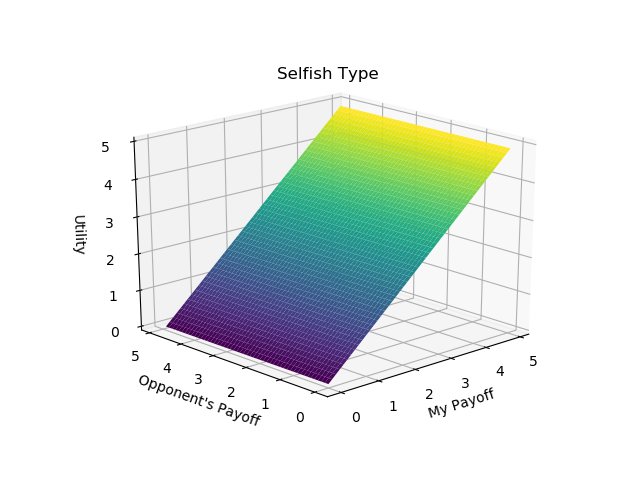
\includegraphics[scale=0.75]{resources/selfish.png}
	\caption{An example of a purely selfish type represented as a `utility surface'.}
	\label{selfishUtilitySurface}
\end{figure}

\begin{figure}
\[
	\begin{bmatrix} 
	0. & 0. & 0. & \dots & 0. & 0. & 0.\\
	0.1 & 0.1 & 0.1 & \dots & 0.1 & 0.1 & 0.1\\
	0.2 & 0.2 & 0.2 & \dots & 0.2 & 0.2 & 0.2\\
	\vdots & \vdots & \vdots & \dots & \vdots &\vdots &\vdots\\
	4.7 & 4.7 & 4.7 & \dots & 4.7 & 4.7 & 4.7\\
	4.8 & 4.8 & 4.8 & \dots & 4.8 & 4.8 & 4.8\\
	4.8 & 4.8 & 4.8 & \dots & 4.8 & 4.8 & 4.8 
	\end{bmatrix}
\]
\caption{A `selfish' utility grid with $\phi = 5$ and $s = 0.1$.}
\label{selfishUtilityGrid}
\end{figure}

\np Phenotypic mutation is performed by creating a small perturbation to the resident surface in a randomly selected area.
We assume this perturbation takes the shape of a bivariate normal distribution with standard deviation $\sigma$, where $\sigma \sim U(0,\gamma)$ and $\gamma$ is a parameter of the model.
This method ensures that mutations are small.
It also has the effect of creating \textit{localised} mutations: mutations that only affect a certain area of the surface rather than the shape of the surface overall.
It turns out that the localised nature of these mutations is important and will be discussed in proceeding sections.
Figure \ref{selfishUtilitySurfaceOneMutation} shows our selfish utility surface from \ref{selfishUtilitySurface} after one mutation has been applied.
\begin{figure}
	\centering
	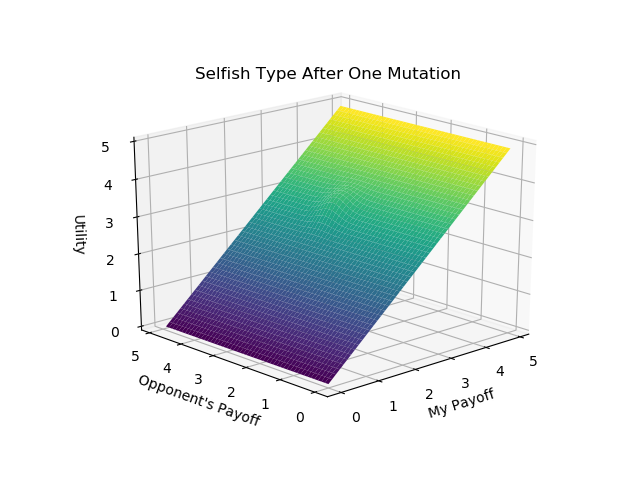
\includegraphics[scale=0.7]{resources/one_mutation.png}
	\caption{The selfish utility surface after one mutation has been applied at the point (3, 3).}
	\label{selfishUtilitySurfaceOneMutation}
\end{figure}
\paragraph{Symbolic Representation}
\np The second method by which we represent individuals is by maintaining the symbolic expression of a two parameter function.
This expression (which is the phenotype) is not the only information stored about each individual though.
An individual also consists of its genome, an array of integers (`codons') that is used to generate the phenotype in conjunction with the grammar.
This representation makes use of the software package of \citet{fenton_ponyge2:_2017}, the documentation of which has in depth explanations of the representation's inner workings.

\np Briefly, the grammar is a set of rules that govern the kinds of individuals that can be generated.
To generate a phenotype, the grammar rules are enumerated with the phenotype iteratively constructed.
Each time a choice is to be made between two or more options, we take the modulo of the current codon by the number of available options, this value is used to select the rule.
The grammar, in Backus-Naur form \citep{oneill_grammatical_2001}, is a parameter of the model and inherently introduces bias into the simulation.
The grammar that was used for the majority of our simulations is shown in \ref{grammar}, where $<o>, <e> and <c>$ are rules and the terms separated by $|$ are the possible results of that rule.
In the grammar, $r$ is used as a stand in the the index of assortativity, $\alpha$.
After initial experimentation, it became clear that adding the index of assortativity as a terminal within the grammar
tended to led to much more meaningful results than if simulations were left to arrive at this value independently.
\begin{figure}[]
	\centering
	\begin{align*}
		&<o> ::= \qquad <e>+<e>|\\
		& \qquad \qquad \qquad <e>-<e>| \nonumber \\
		& \qquad \qquad \qquad <e>*<e>| \nonumber \\ \nonumber \\
		&<e> ::= \qquad <e>+<e>| \nonumber \\
		&\qquad \qquad \qquad <e>-<e>| \nonumber \\
		&\qquad \qquad \qquad <e>*<e>| \nonumber \\
		&\qquad \qquad \qquad <c><c>.<c><c>| \nonumber \\
		&\qquad \qquad \qquad r| \nonumber \\
		&\qquad \qquad \qquad myPayoff| \nonumber \\
		&\qquad \qquad \qquad opponentPayoff \nonumber \\ \nonumber \\
		&<c>  ::= \qquad 0 | \quad 1 |\quad 2 |\quad 3 |\quad 4 |\quad 5 |\quad 6 |\quad 7 |\quad 8 |\quad 9 \nonumber
	\end{align*}
\caption{The grammar in BNF form, used to govern the generation of individuals in Symbolic Representation. Where $r$ is a stand in for the index of assortativity, $\alpha$}
\label{grammar}
\end{figure}


\np Mutation is performed by modifying integers within the genome of individuals.
When a mutation occurs, the integer of each codon within the genome is randomly altered.
This way, when the grammar is traversed again to generate the phenotype and the codons are used to select between options, different codons will produce different outcomes.

\np Unlike the Phenotype Representation, this method of representing individuals results in utility functions that are continuous and un-bounded in terms of the size of the payoffs that it can interpret.
However, Symbolic Representation comes with the significant drawback of the grammar encoding bias into the model.
It is difficult to overstate the importance the grammar has on the dynamics of the system.
Another point of difference is that mutations in this case affect the function overall, rather than a specific area of the space.
So, with Symbolic Representation, there is no concept of the `locality' of the mutation - mutations affect the whole space.

\todo{is here the place to talk about results of choosing a bad grammar?}


\section{Measuring Success}\label{success}
It is difficult to analyse the results of the two different methods we're using in the same way.
So, for each of the two representations we will look at two different measures to assess the results.
One, is some measure of similarity between the phenotypes of the evolved individuals and the phenotype of the prediction made by \citet{alger_generalization_2012}.
The second is a comparison of the behaviour of the evolved individuals against that of the predicted function.

\np In the case of Phenotype Representation, given the way mutation operates and since we are confined by the $\phi$ parameter, 
the individuals produced by the simulation exist approximately within the confines of a $(\phi \times \phi \times \phi)$ cube.
So, we can compare the individuals based on the volume of the space between the two surfaces (evolved and predicted).
This is not a comparison of total volume of the surfaces.
Rather, it is a sum of the point-by-point absolute difference between the two surfaces.
In the proceeding, this measure will be referred to as the `volume-difference'.

\np This volume-difference is not helpful when analysing the results of Symbolic Representation.
This is because an evolved function can be shifted along the z-axis (the utility-axis) by the addition (subtraction) of some constant.
This constant changes the utility-values produced by the function and so changes the potential volume-difference but does not alter the outcomes that the individual prefers.
This is illustrated in the following:

	\begin{alignat*}{2}
	u & > u_i \\
	u + c & > u_i +c
	\end{alignat*}

Where $u$ and $u_i$ are utility values produced by an individual's utility function and c is some constant.
However, since in the symbolic case we have the expression of the function, we can analyse this function directly to compare its similarity with the AW prediction.

\np Finally, in both cases we can look at the fitness of the evolved individuals.
By comparing the average payoff earned by the evolved individuals when playing against the AW prediction, with that earned the AW prediction playing against itself, we can get a measure of the similarity of behaviour.
If our evolved indiviuduals are similar to the prediction, we would expect them to prefer similar outcomes and hence achieve an average payoff when playing against the prediction, similar to what the prediction achieves playing against itself.
In this context average payoff (and by extent fitness) is not intended to be an indicator of the reproductive success of an individual but rather a measure of the similarity of preferences.

\section{Putting it all together}

Along with the wider context presented in Chapter \ref{lit_review}, now have the key elements of the framework that will be used to perform experiments.
These include an understanding of the fitness measure and the kinds of games that will be played in performing this measure.
As well as the details of the different methods of representing individuals we will explore.
Finally, from \ref{success}, we have understanding of some of the methods that will be used in analysing results.
Before we begin presenting and discussing these results, we lay out how the rest of the thesis is organised.

\np We begin in the next chapter, Chapter \ref{symmetricGames}, with an exploration of the results generated by running simulations with symmetric games.
Firstly, in section \ref{symmetricGames_pheno} we detail the outcomes of the Phenotype Representation simulations.
Before continuing with a presentation of the results of the Symbolic Representation simulations in \ref{symmetricGames_symb}.

\np In Chapter \ref{asymmetricGames} we move beyond the scope of the \citeauthor{alger_generalization_2012} work by exploring asymmetric games.
We again begin with the results of the Phenotype Representation, with the results of Symbolic Representation presented in the proceeding section.
The key insights of these results are then discussed in Chapter \ref{discussion}.


\chapter{Symmetric Games}\label{symmetricGames}

We begin with simulations in which individuals are paired to play symmetric, two player games.
This model aligns closely with the results of \citet{alger_generalization_2012}.
So, we are here exploring how the dynamics of a system that adheres to the assumptions made by AW affect the models convergence to the prediction made by AW.
We also implement the assortative matching of AW to investigate how this affects the individuals that are produced by simulation.

\section{Phenotype Representation}\label{symmetricGames_pheno}
Using the technique just described in section \ref{representing_mutating}, we simulate evolution operating at the level of the phenotype.
Fitness is a product of the individual's performance in many symmetric games.
Starting with a randomly generated surface, we run simulations with the following parameters:
\begin{gather*}
	\phi = 5\\
	s = 0.1\\
	\alpha = 0\\
\end{gather*}
\noindent When $\alpha = 0$, the function predicted by \citet{alger_generalization_2012} equates to pure selfishness.
So we are interested in how closely the surface produced by our dynamically evolving system aligns to a surface of pure selfishness.
Figure \ref{average_r_0_symmetric_evolved} shows an average of the surfaces that resulted from ten simulations with these parameters.
Looking at this figure and comparing it to figure \ref{selfishUtilitySurface}, it is not obvious that there is a huge amount of similarity between the two.
This is confirmed measuring the difference in volume between the evolved surfaces and pure selfishness. 

\np The volume-difference between the average surface and the predicted is 19.112 (for context the total volume between the selfish surface and the zero-plane is 62.5).
This difference tends to increase if we look at the volume-difference between each of 10 surfaces individually and selfishness.
Figure \ref{boxplot_volume_difference_symmetric} displays these measures.
There tends to be a volume-difference of about a third of the total volume of the selfish surface between the evolved surfaces and the selfish surface.

\begin{figure}
	\centering
	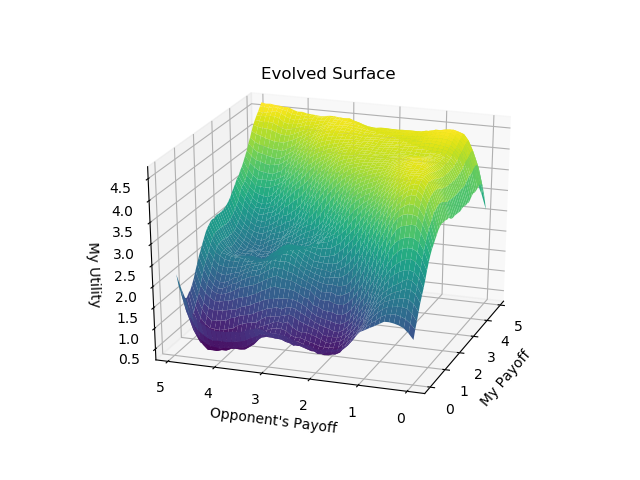
\includegraphics[scale=0.7]{resources/average_r_0_symmetric_evolved.png}
	\caption{An average of the surfaces evolved by symmetric-game, Phenotype Representation when $\alpha = 0$.}
	\label{average_r_0_symmetric_evolved}
\end{figure}

\np Performing similar analysis on the surfaces evolved when $\alpha \neq 0$ yields similar results.
The figure \ref{average_r_03_symmetric_evolved} shows the average evolved surface when $\alpha = 0.3$.
The volume-difference between this surface and the evolved surface when $\alpha = 0$ - shown in figure \ref{average_r_0_symmetric_evolved} - is so small as to be negligible.
This is notable the AW prediction differs significantly depending on $\alpha$.
As before, we can also look at the volume-differences between the surfaces produced by the simulation and the AW prediction.
Figure \ref{boxplot_volume_difference_symmetric} shows the distribution of these volumes, the volume-difference between the average surface and the AW prediction is 23.282.
Now that $\alpha$ is greater than zero and AW predicts some level of cooperation between individuals, our evolved surfaces are even more dissimilar to the AW prediction.

\begin{figure}
	\centering
	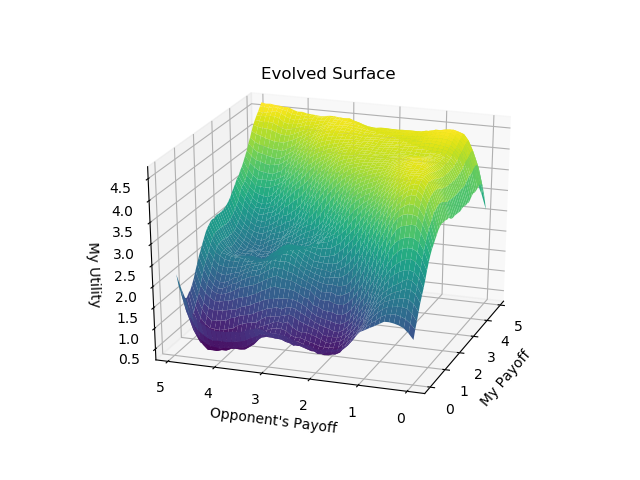
\includegraphics[scale=0.7]{resources/average_r_03_symmetric_evolved.png}
	\caption{An average of the surfaces evolved by symmetric-game, Phenotype Representation when $\alpha = 0.3$.}
	\label{average_r_03_symmetric_evolved}
\end{figure}

\begin{figure}
	\centering
	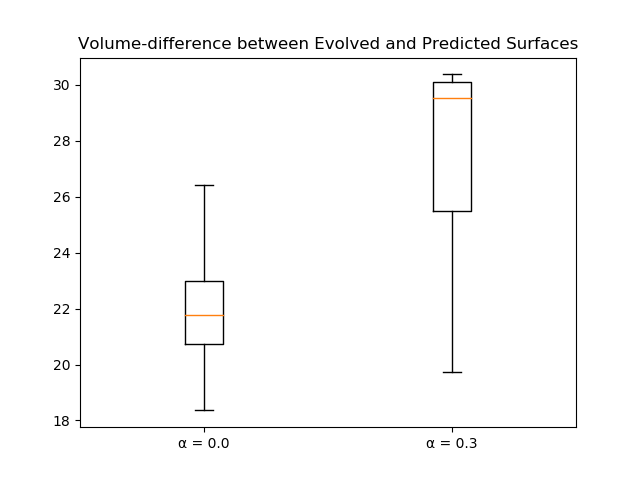
\includegraphics[scale=0.6]{resources/distance_boxplot_r_00_03.png}
	\caption{Volume-differences between each of the evolved surfaces and the AW prediction. Calculated for $\alpha = 0$ and $\alpha = 0.3$.}
	\label{boxplot_volume_difference_symmetric}
\end{figure}


\np So, our evolved surfaces are not overly similar to the prediction made by AW surface in terms of volume-difference, but how do they fare in terms of fitness?
Figure \ref{phenotype_barchart_fitness_earned_against_target_r_00_03} shows the fitnesses earned by the average evolved surface when playing against the AW predicted surface.
Rather than being a measure of reproductive success, the fitness here is intended to highlight the difference in \textit{behaviour} between the evolved and predicted surfaces.
If the evolved surfaces were qualitatively similar to the AW prediction, we would expect the fitness earned by the evolved surface playing against the predicted surface to approach that earned by the predicted surface playing against itself.
But is does not occur.
In both instances, the fitness earned by the evolved surface differs from the expected fitness.

\np It is interesting though, that the evolved surfaces seem to out-perform the predicted surface.
So even though the evolved surfaces are different from the AW prediction, perhaps our simulations have arrived at something that can invade the surfaces entailed by this prediction?
Figure \ref{linegraph_fitness_difference_increasing_epsilon} shows the difference in personal fitness earned by the evolved surface against the AW prediction as the proportion of the population  that is the evolved surface increases.
In this figure, a positive number on the \textit{y-axis} indicates that evolved surface has achieved a higher fitness increase than the AW prediction.
The positive `fitness difference' values to the left this figure indicate that when the AW prediction is the resident in a population and our average-evolved surface enters this population,
the evolved surface achieves a higher personal payoff than the prediction when the proportion of the population that is the evolved type is low.
As this proportion increases though, the fitness difference moves back in favour of the AW predication, and so our evolved surface will not be able to invade.
This is in agreement with AW's prediction.
\begin{figure}
	\centering
	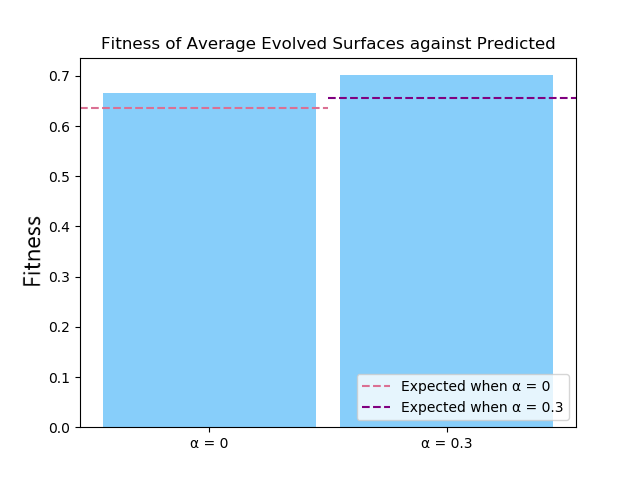
\includegraphics[scale=0.6]{resources/phenotype_barchart_fitness_earned_against_target_r_00_03.png}
	\caption{Fitness earned by average evolved surface against the predicted surface, compared with the expected fitness; i.e. the fitness earned by the predicted surface playing against itself. Calculated for $\alpha = 0$ and $\alpha = 0.3$.}
	\label{phenotype_barchart_fitness_earned_against_target_r_00_03}
\end{figure}
\begin{figure}
	\centering
	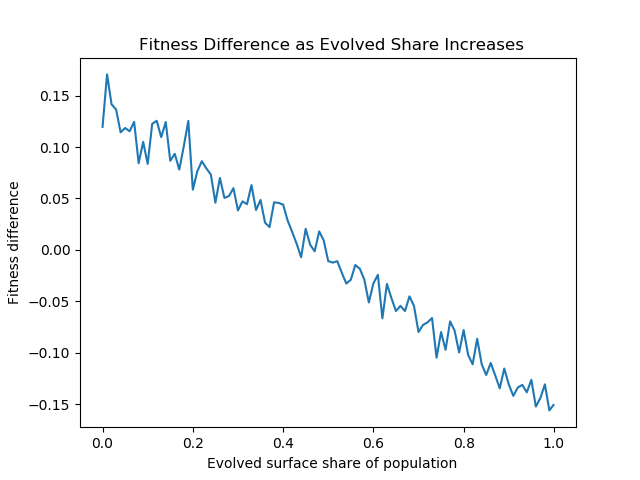
\includegraphics[scale=0.7]{resources/linegraph_fitness_difference_increasing_epsilon.png}
	\caption{Fitness difference between evolved surface and predicted surface; $\alpha = 0$.
	When $\epsilon$ is small, the evolved surface achieves a greater fitness than the predicted surface, but as $\epsilon$ grows the predicted surface achieves a greater fitness.
	This indicates that no invasion will occur.}
	\label{linegraph_fitness_difference_increasing_epsilon}
\end{figure}
\np Phenotype Representation with symmetric games has not been able to recover the results of \citet{alger_generalization_2012}.
We did though, converge towards an interesting surface that performed reasonably well in fitness evaluation.
This well-performing surface allowed us to investigate the evolutionary stability of the AW prediction which we were not able to create a counter-example to. 
It is possible that this method of mutation has produced surfaces that are on their way to converging on an alternative evolutionary stable function.


\section{Symbolic Representation}\label{symmetricGames_symb}

We now turn our attention to our second method of representing individuals.
We start with a randomly generated genome, and simulate evolution via the technique described in section \ref{representing_mutating}.
In the case of Symbolic Representation, it is a little more difficult to give a general picture of the kinds of functions that evolved than it is in the phenotypic case.
Since small mutations in genome can lead to vastly different utility values being generated by the function (e.g. a $+$ becomes a $\times$), it does not make sense to think of an average function that is generated,
but we can think about the kinds of functions that are generated.

\np Considering one group of ten simulations, where $\alpha = 0$, seven of the evolved functions correspond exactly to pure selfishness,
while one contains reference to the payoff earned by the opponent, the utility is heavily slanted towards selfishness.
Finally, two of the resultant functions can be considered noise.
These results and the corresponding functions are displayed in figure \ref{barchart_fitness_earned_against_target_r_00}.
The dashed, threshold-line in this figure is the fitness earned by Pure Selfishness when playing against itself.

\np It can quickly be seen that functions $f$ and $g$ are poorest performing functions of the group.
This is makes sense when the functions themselves are considered: in generating a utility value neither function takes into account the player's payoffs.
For example, given that $\alpha=0$, functions $d$ and $h$ both reduce down to pure selfishness.
Another point to note is that functions $b$ and $i$, for example, result in exactly the same behaviour because the slopes of the resultant surfaces are equal.
The utility value generated by a particular function has no meaning if compared to the value generated by another individual.
Utility only carries weight when it is compared to another utility value of the same individual. 


\begin{figure}
	\centering
	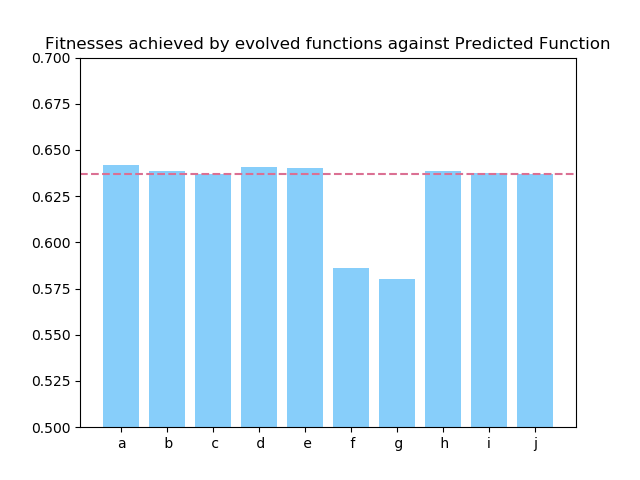
\includegraphics[scale=0.7]{resources/ylim_barchart_fitness_earned_against_target_r_00.png}
	\begin{alignat*}{2}
		a: f(x, y) = & 12.37x - y + \alpha &\\
		b: f(x, y) = & x + 70.54&\\
		c: f(x, y) = & 47.17x - 46.68&\\
		d: f(x, y) = & x + 1251.2448\alpha y&\\
		e: f(x, y) = & x + \alpha &\\
		f: f(x, y) = & 31.38\alpha &\\
		g: f(x, y) = & 34.68\alpha &\\
		h: f(x, y) = & x + x^2y^2\alpha &\\
		i: f(x, y) = & x - 97.58&\\
		j: f(x, y) = & x + 48&\\
	\end{alignat*}
	\caption{Fitness earned by each evolved function when playing against AW prediction alongside the corresponding functions; where $x$ is the payoff earned by the owner of utility function, y is the payoff earned by their opponent and $\alpha = 0$.}
	\label{barchart_fitness_earned_against_target_r_00}
\end{figure}

\np With no assortativity in the matching process, Symbolic Representation seems to converge towards the selfishness predicted by AW,
but we'll see now that things are a little more complicated when assortativity is introduced.

\begin{figure}
	\centering
	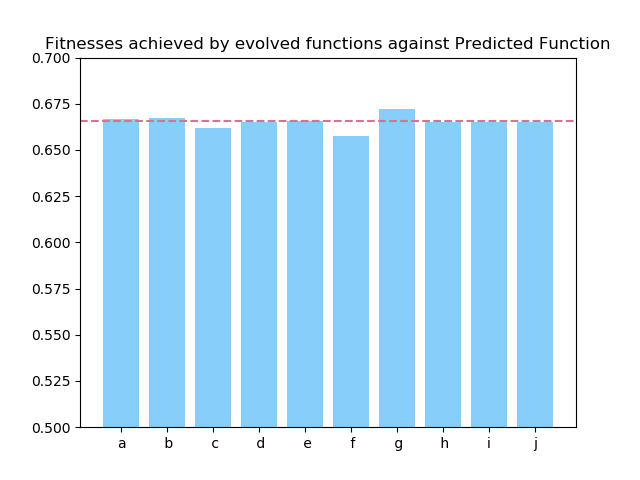
\includegraphics[scale=0.7]{resources/ylim_barchart_fitness_earned_against_target_r_06.png}
	\begin{alignat*}{2}
		a: f(x, y) = & 2.9339x + \alpha y&\\
		b: f(x, y) = & x + \alpha y -\alpha &\\
		c: f(x, y) = & 199082.093x + 3.02&\\
		d: f(x, y) = & 2x + y&\\
		e: f(x, y) = & x^3 + (\alpha^2 + 81.45)x + (\alpha+42.48)y + 2\alpha &\\
		f: f(x, y) = & 11.03x&\\
		g: f(x, y) = & (\alpha + 56.95)x^2 - 2x + 26.75y^2  + (\alpha^2 - 0.65)y  - \alpha^2 + \alpha + 130.38&\\
		h: f(x, y) = & 78.35(\alpha^2)(x^2) + (1 +74.62\alpha )y + \alpha + 1.11&\\
		i: f(x, y) = & \alpha (x^2) + y + \alpha + 21.64&\\
		j: f(x, y) = & 3x + 2y&\\
	\end{alignat*}
	\caption{Fitness earned by each evolved function when playing against AW prediction alongside the corresponding function; where $x$ is the payoff earned by the owner of utility function, y is the payoff earned by their opponent and $\alpha = 0.6$.}
	\label{barchart_fitness_earned_against_target_r06}
\end{figure}

\np We now run the same simulations, again beginning with a randomly generated genome, with $\alpha = 0.6$.
The evolved functions and the fitness achieved by each function when playing against the AW prediction is shown in figure \ref{barchart_fitness_earned_against_target_r06}.
In this case, only one simulation produced a function that exactly aligns with the AW prediction, function $b$.
\np The figure shows that while largely the simulations have not converged to functions that completely align with the AW prediction,
the behaviour of the individuals in fitness interactions can be relatively similar.
Now that there is some assortativity in the matching process, the functions produced become more unwieldy and complex.in, the simplified evolved functions are displayed the motivation for this is to highlight the fact that now that there is some assortativity in the matching process, the functions produced become more unwieldy and complex.
However, simplifying the functions can show that they're more similar to the AW predication than they first appear.
It seems that where the simulation has been unable to produce a function that exactly matches the AW prediction, the individuals have tended towards approximations.
Function $j$ is a good example of this.
When $\alpha = 0.6$, the AW function predicts that an individual who values their opponent's payoff with 0.6 the weight that they value their own will result in ESS play.
Since we are interested in the ratio of the weight attributed to each players payoff, we can rewrite function $j$ as:
\begin{equation*}
	f(x, y) = x + \frac{2}{3} y
\end{equation*}


\noindent Which is a quite close approximation of the AW prediction.
The same can be said of $d$, which associates a weight of $0.5$ to the opponent's payoff, again a relatively good approximation of the $0.6$ that was predicted by AW.

\np This difficulty in converging to the exact AW prediction that arises when $\alpha \neq 0$, could be because the function we're attempting to evolve in this case is more complicated than finding an equivalent to pure selfishness.
There are just more ways to arrive at an equivalent of selfishness than there are at an equivalent of \ref{linearESSEquation}, and so we see the simulations more easily converge in the case when $\alpha = 0$.


\np Having now presented results relating to symmetric games and analysed there similarity to the AW prediction we now move beyond the scope of this work.
The next chapter focusses on results of simulations in which individuals are matched to play asymmetric games.
This juxtaposition of results generated by symmetric and asymmetric games will allow us to explore how symmetry has affected the dynamics how our system.
Further, we will be able to investigate how heavily the results of \citeauthor{alger_generalization_2012} rely on their assumption of symmetry.

\chapter{Asymmetric Games}\label{asymmetricGames}
We now turn our attention to simulations in which individuals are paired to play asymmetric, two player games.
Because of this, the simulations discussed in this chapter align less closely with \citet{alger_generalization_2012} than those in the preceding chapter.
However, we maintain our implementation of assortative matching to investigate how this affects the individuals that are produced by simulation.
As before, we begin with the results of the Phenotype Representation before moving on to the Symbolic Representation.


\section{Phenotype Representation}\label{asymmetricGames_pheno}
Using the same technique as used in symmetric case, section \ref{symmetricGames_pheno}, we simulate evolution operating at the level of the phenotype.
Now, fitness is a product of the individual's performance in many asymmetric games.
Starting with a randomly generated surface, we run simulations with the following parameters:

\begin{gather*}
	\phi = 5\\
	s = 0.1\\
	\alpha = 0\\
\end{gather*}

When $\alpha = 0$, we would expect the evolved surfaces to converge towards pure-selfishness.
Just looking at figure \ref{average_r_0_asymmetric_evolved} we can see that it seems to be somewhat similar pure-selfishness.
This observation is confirmed by the volume-difference, which for the average evolved surface (against selfishness) is 11.9657, so an improvement on the symmetric case's 19.112.
Despite have some level of assortativity in the matching, $\alpha = 0.4$, figure \ref{average_r_04_asymmetric_evolved} too shows a surface that resembles pure-selfishness.
This average evolved surface does not fair well when compared against the AW prediction, with a volume-difference of 29.3766.
Surprisingly though, this surface - evolved with $\alpha = 0.4$ - is a close approximation of pure-selfishness.
The average evolved surface when $\alpha = 0.4$ has a volume-difference of 13.9255 with pure-selfishness.

\begin{figure}
	\centering
	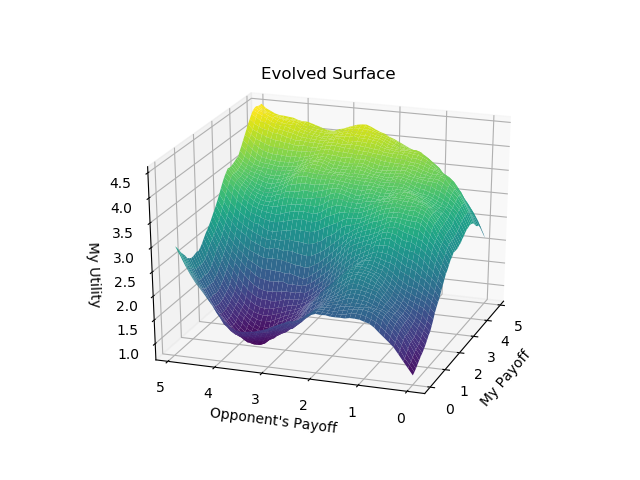
\includegraphics[scale=0.7]{resources/asymmetric_average_evolved_surface_r_00.png}
	\caption{An average of the surfaces evolved by asymmetric-game, Phenotype Representation when $\alpha = 0$.}
	\label{average_r_0_asymmetric_evolved}
\end{figure}

\begin{figure}
	\centering
	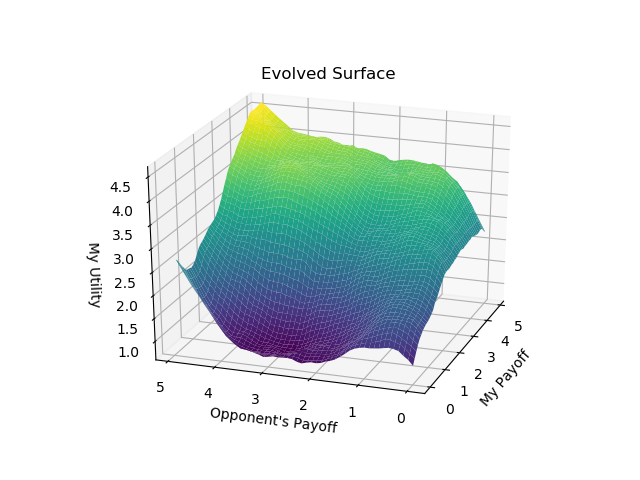
\includegraphics[scale=0.75]{resources/asymmetric_average_evolved_surface_r_04.png}
	\caption{An average of the surfaces evolved by asymmetric-game, Phenotype Representation when $\alpha = 0.4$.}
	\label{average_r_04_asymmetric_evolved}
\end{figure}

\np The volume-differences calculated for each evolved surface individually are shown in figure \ref{asymmetric_distance_boxplot_r_00_04}.
The distribution of volume-differences for the surfaces generated when $\alpha = 0$ indicate that this kind of simulation has produced surfaces that are consistently shifting towards pure-selfishness.
What is interesting though is that the AW prediction does not seem to hold when games are asymmetric assortativity is introduced into the matching process.


\begin{figure}
	\centering
	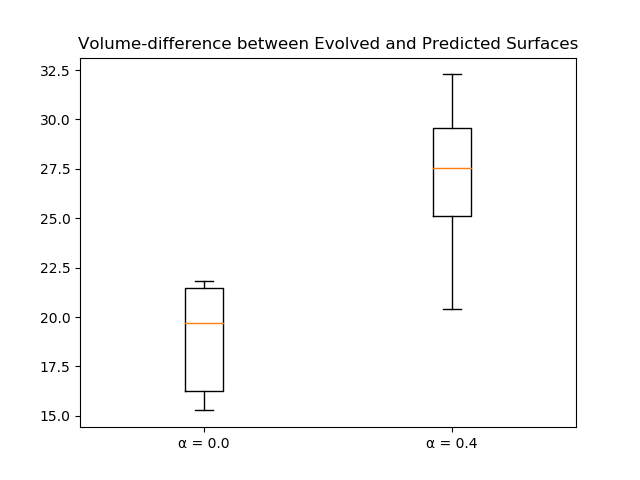
\includegraphics[scale=0.6]{resources/asymmetric_distance_boxplot_r_00_04.png}
	\caption{Volume-differences between each of the evolved surfaces and the AW prediction. Calculated for $\alpha = 0$ and $\alpha = 0.4$.}
	\label{asymmetric_distance_boxplot_r_00_04}
\end{figure}



\section{Symbolic Representation}\label{asymmetricGames_symb}
We now look again at the results of simulations run with Symbolic Representation.
We start with a randomly generated genome, and simulate evolution via the technique described in section \ref{representing_mutating}.
Fitness is determined by the individuals performance in many asymmetric games.
As with section \ref{symmetricGames_symb}, we evaluate our evolved functions by assessing their behaviour when playing against the target.
Further to this, we can assess the functions themselves.
Figure \ref{asymmetric_barchart_fitness_earned_against_target_r00} shows the fitness achieved by function evolved with $\alpha = 0$ when playing against the AW prediction as well the functions themselves.

\begin{figure}
	\centering
	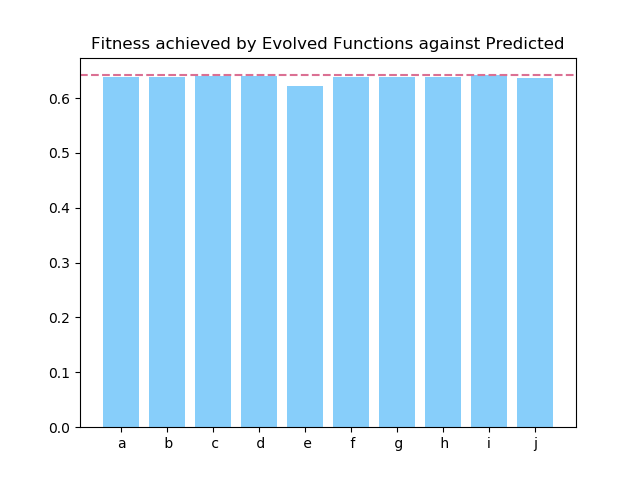
\includegraphics[scale=0.7]{resources/ylim_barchart_fitness_earned_against_target_asymmetric_r_00.png}
	\begin{alignat*}{2}
		a: f(x, y) = & x - 59.61&\\
		b: f(x, y) = & x - 77.15&\\
		c: f(x, y) = & x + \alpha &\\
		d: f(x, y) = & x - \alpha &\\
		e: f(x, y) = & xy - \alpha y - \alpha  - y + 82.42&\\
		f: f(x, y) = & x - \alpha &\\
		g: f(x, y) = & 98.13 + 58.67x&\\
		h: f(x, y) = & 2x - \alpha y + 90\alpha &\\
		i: f(x, y) = & 1583.5408\alpha xy^2+x+25.17\alpha ^2x&\\
		j: f(x, y) = & x-\alpha ^2&\\
	\end{alignat*}
	\caption{Fitness earned by each evolved function when playing against AW prediction alongside the corresponding function; where $x$ is the payoff earned by the owner of utility function, y is the payoff earned by their opponent and $\alpha = 0.0$.}
	\label{asymmetric_barchart_fitness_earned_against_target_r00}
\end{figure}
\np Given that $\alpha = 0$ we would expect the functions to converge towards pure selfishness.
This has occurred in all but one of the simulations (function $e$).
The convergence towards selfishness has slightly increased in this asymmetric case compared to the symmetric.
These results are confirmed by the fitnesses displayed in figure \ref{asymmetric_barchart_fitness_earned_against_target_r00}.

\np Looking at the functions generated when $\alpha = 0.6$, we see a similar trend to the one we saw when assortativity was introduced in the symmetric case.
Like in the symmetric case we see an increased complexity in the evolved functions when assortativity is introduced.
However, now that we're sampling asymmetric games it this effect has increased.
Not only that but not one of our ten simulations has converged to the prediction.
Functions $a$ and $b$ have though landed on an approximation of the AW prediction, given that these simulations have landed on a function that assigned a weight of $0.5$ to their opponent player.


\begin{figure}
	\centering
	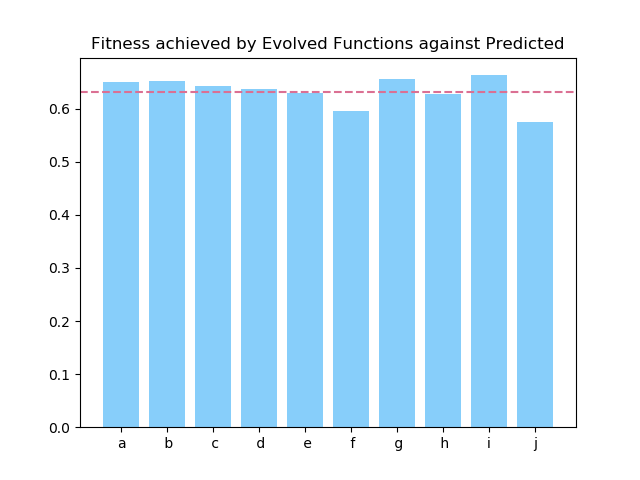
\includegraphics[scale=0.7]{resources/ylim_barchart_fitness_earned_against_target_asymmetric_r_06.png}
	\begin{alignat*}{2}
		a: f(x, y) = & 2x + y\\
		b: f(x, y) = & 23.83yx^2 - 2x + (1 - r - r^3)y - 4.94r^3 + 56.43r ^2 + 2r - 451.1485\\
		c: f(x, y) = & 09.06\alpha x + yx\\
		d: f(x, y) = & x - \alpha + 4512.086\\
		e: f(x, y) = & 2x + y\\
		f: f(x, y) = & x+87.82\\
		g: f(x, y) = & 86.69*x\\
		h: f(x, y) = & 30.84\alpha x - 2\alpha y +\alpha + 3.359\\
		i: f(x, y) = & 203.1086*y*x^2 +(\alpha - 42.36)x + 62.30y^2 - 2y  -2\alpha -239.28\\
		j: f(x, y) = & 39.51\alpha xy^2 + (94.59\alpha^3 - \alpha^2)x + (35.07 + 75.67\alpha)y - 3\alpha - 91.41\\
	\end{alignat*}
	\caption{Fitness earned by each evolved function when playing against AW prediction alongside the corresponding function; where $x$ is the payoff earned by the owner of utility function, y is the payoff earned by their opponent and $\alpha = 0.6$.}
	\label{barchart_fitness_earned_against_target_asymmetric_r_06}
\end{figure}


\chapter{Discussion}\label{discussion}

Having presented the results of the simulations we now discuss the interesting conclusions that can be drawn and 
\todo{finish intro one section done.}


\section{Symbolic Representation: A Path to Selfishness}
The results presented regarding the simulations run with the Symbolic Representation in both Chapters \ref{symmetricGames} and \ref{asymmetricGames} 
When $\alpha = 0$, sixteen out the twenty simulations (combining symmetric and asymmetric runs) produced functions that were equivalent to pure selfishness.
This aligns with the AW prediction. 


\section{Phenotype Representation: In It To Win It}\label{win_it}
\np Perhaps the most puzzling result presented in the preceding two chapters is the output of simulations using Phenotype Representation and sampling symmetric games.
These results, detailed in section \ref{symmetricGames_pheno}, show that this kind of simulation produces individuals
 that derive higher utility when their payoffs are greater than their opponent's.
Individuals with this utility function are indifferent as to how much greater their payoff is, or indeed the size of their payoff at all: as long as it is greater than that achieved by their opponent.
This result cannot be attributed solely to the effect of sampling symmetric games, because these results are not mirrored in the functions generated by the Symbolic Representation simulations (section \ref{symmetricGames_symb}).
Nor can we say that the Phenotype Representation accounts for these results: sampling asymmetric games produces surfaces that are more aligned with our expectations of pure selfishness.
The hypothesis is that this divide along the identity line is a product of sampling only symmetric games in conjunction with the localised mutations of the Phenotype Representation.

\np In essence, when games are symmetric, each interaction that a resident and mutant engage in occurs across the identity line in the payoff point space.
There are two payoff points exactly on the line, $[a,a]$ and $[d,d]$.
And the other two point occur (symmetrically) on either side of the line, $[b,c]$ and $[c,b]$.
Arbitrarily, let's say that $b \geq c$.
Since the payoff earned by each player is equal, payoff points that are on the line of equality ($[a,a] \& [d,d]$) do not contribute to a difference in fitness, so can be ignored.
The other two payoff points in a given game are where the difference in fitness between the individuals is determined.
Since the points $[a,a]$ and $[d,d]$ do not contribute to a difference in fitness, no matter how large a payoff can be earned evolution will be indifferent towards preferences that lead to these outcomes.
Instead, evolution will favour only preferences that lead the individual to earn \textit{payoff b}.
By definition, this payoff point is always on the same side of the identity line, i.e. the side of the line in which the payoff earned by the individual is greater than that earned by their opponent.
So mutations that lead to the individual preferring outcomes that are situated on this side of the identity line will be more reproductively successful.

\np The other factor at play here is the kind of mutations that are performed with the Phenotype Representation detailed in section \ref{representing_mutating}.
As mentioned in the initial discussion, these mutation are \textit{local}.
They do not affect the structure of the utility function or overall change to way that the function deals with the payoffs generally.
Rather, if a mutation occurs at the point $(i, j)$ in the utility space only preferences regarding outcomes that are close to this point will be altered.
In other words, preferences about the event in which the individual earns a payoff close to $i$ and their opponent earns a payoff close to $j$.
If the point $(i, j)$ is on the same side of the identity line as payoff b, and the mutation that occurs at this point makes this outcome more preferable to the individual, then likely this mutation will be accepted.
The converse is true if the mutation is makes this outcome less preferable to the individual, or if the point $(i, j)$ occurs on the opposite side of the identity line.

\np This analysis of payoff structures is relatively straight-forward.
We are accustomed to thinking about evolution as favouring individuals who are \textit{better} somehow than their opponents. 
But this kind of mutation coupled with symmetric games has produced a kind of \textit{minimal-betterness} that requires individuals achieve only-just more than their counter-parts.
As their opponents achieve more, the individual must also achieve a little more and as the opponent achieves less, the individual is able to achieve less also.
It seems that we may have developed a utility function has over-adapted to the simulation rather than a function that will be generally evolutionarily successful.
Having said that, this would be a utility function that has over-adapted to the assumptions made in \citet{alger_generalization_2012}.


\section{Evolutionary Stability: An Alternate Destination}
Staying with the symmetric-game Phenotype Representation, an additional interesting point regarding the results of these simulations is that they seem to be qualitatively different to the AW prediction.
Where the results of the Symbolic Representation and the asymmetric games sampling seem to approach the AW prediction with varying degrees of success, surfaces generated by symmetric-game Phenotype Representation are converging towards something different.
It is possible that the state that the surfaces are converging towards is an alternative candidate for evolutionary stability.

\np The AW prediction that has been referenced throughout this work is shown in equation \ref{linearESSEquation}.
The conclusions that Alger and Weibull draw regarding this result are only concerned with its evolutionary stability.
Not whether its status as an evolutionary stable utility function is exclusive.
It is possible that other function types exist that are also evolutionarily stable.
It is possible that the surface that our symmetric-game Phenotype Representation is converging towards is one of them.

\np Figure \ref{linegraph_fitness_difference_increasing_epsilon} 
shows how the fitness difference when our evolved surface plays against pure-selfishness is in favour of the evolved surface when the evolved surface only makes up a small proportion of the population.
This difference then steadily moves back in favour of the resident, selfish function as this proportion increases.
This figure is presented to highlight that the evolved surface would not be able to invade the resident AW prediction.
However, the downward slope of the fitness difference is almost perfectly linear as the evolved share of population increases.
When this share is close to 0.5, the fitness difference crosses to be in favour of the AW prediction.

\np As much as this figure can highlight that the AW prediction holds, and cannot be invaded, it could also be indicative of two alternative outcomes.
The first is that given that the predicted surface performs well when its share of the population is low in the saw way that the evolved surface does when it is in the minority,
we may be able to take this as evidence that our evolved surface will be difficult to invade also.
The second is that the change in which function is successful in the fitness comparison happens when the share of population is close to 0.5,
and so there is potentially a mixed type ESS state that is a population consisting of some share of both of these two utility functions.

\todo{check this}


\section{Travels with Randomness}
 > randomness of asymmetric games allows us to explore more?a


\section{Axioms of Preferences}

 > axioms of preferences.




\section{Games Matter}

\todo{Review this section after results are written to see where (if?) it fits}

One of the things that we learn by subjecting the described phenotype to evolution is that the kinds of games that are used to evaluate the fitness of individuals are important.
We begin with a model that uses only a single kind of game to evaluate the fitness of individuals.
Next we move to a conception of fitness that is an aggregation of individuals performance in many different kinds of games.
We explore this evaluation in the symmetric and asymmetric case in chapters \ref{symmetricGames} and \ref{asymmetricGames} respectively.

\paragraph{Single-Game Fitness Measure}
\np In \ref{experimentalFramework} we discuss an approach in which individual fitness is determined based off  how the types perform in one common kind of non-cooperative game, namely prisoner's dilemma.
Using the game structure defined in figure \ref{symmetricGame} we can construct a prisoner's dilemma by setting the following payoffs:
\begin{gather*}
	a = 3\\
	b = 0\\
	c = 4\\
	d = 1
\end{gather*}

\np When running simulations in which each type's fitness is determined by their expected payoff when playing the above game,
it becomes clear that only mutations that occur near to the payoff points ever lead to invasions. 
The payoff points are the four potential outcomes (in terms of payoffs for each player) of the game: (3,3), (0,4), (4, 0) \& (1, 1).
Plotted in figure \ref{prisoners_payoff_plot}.
\begin{figure}
	\centering
	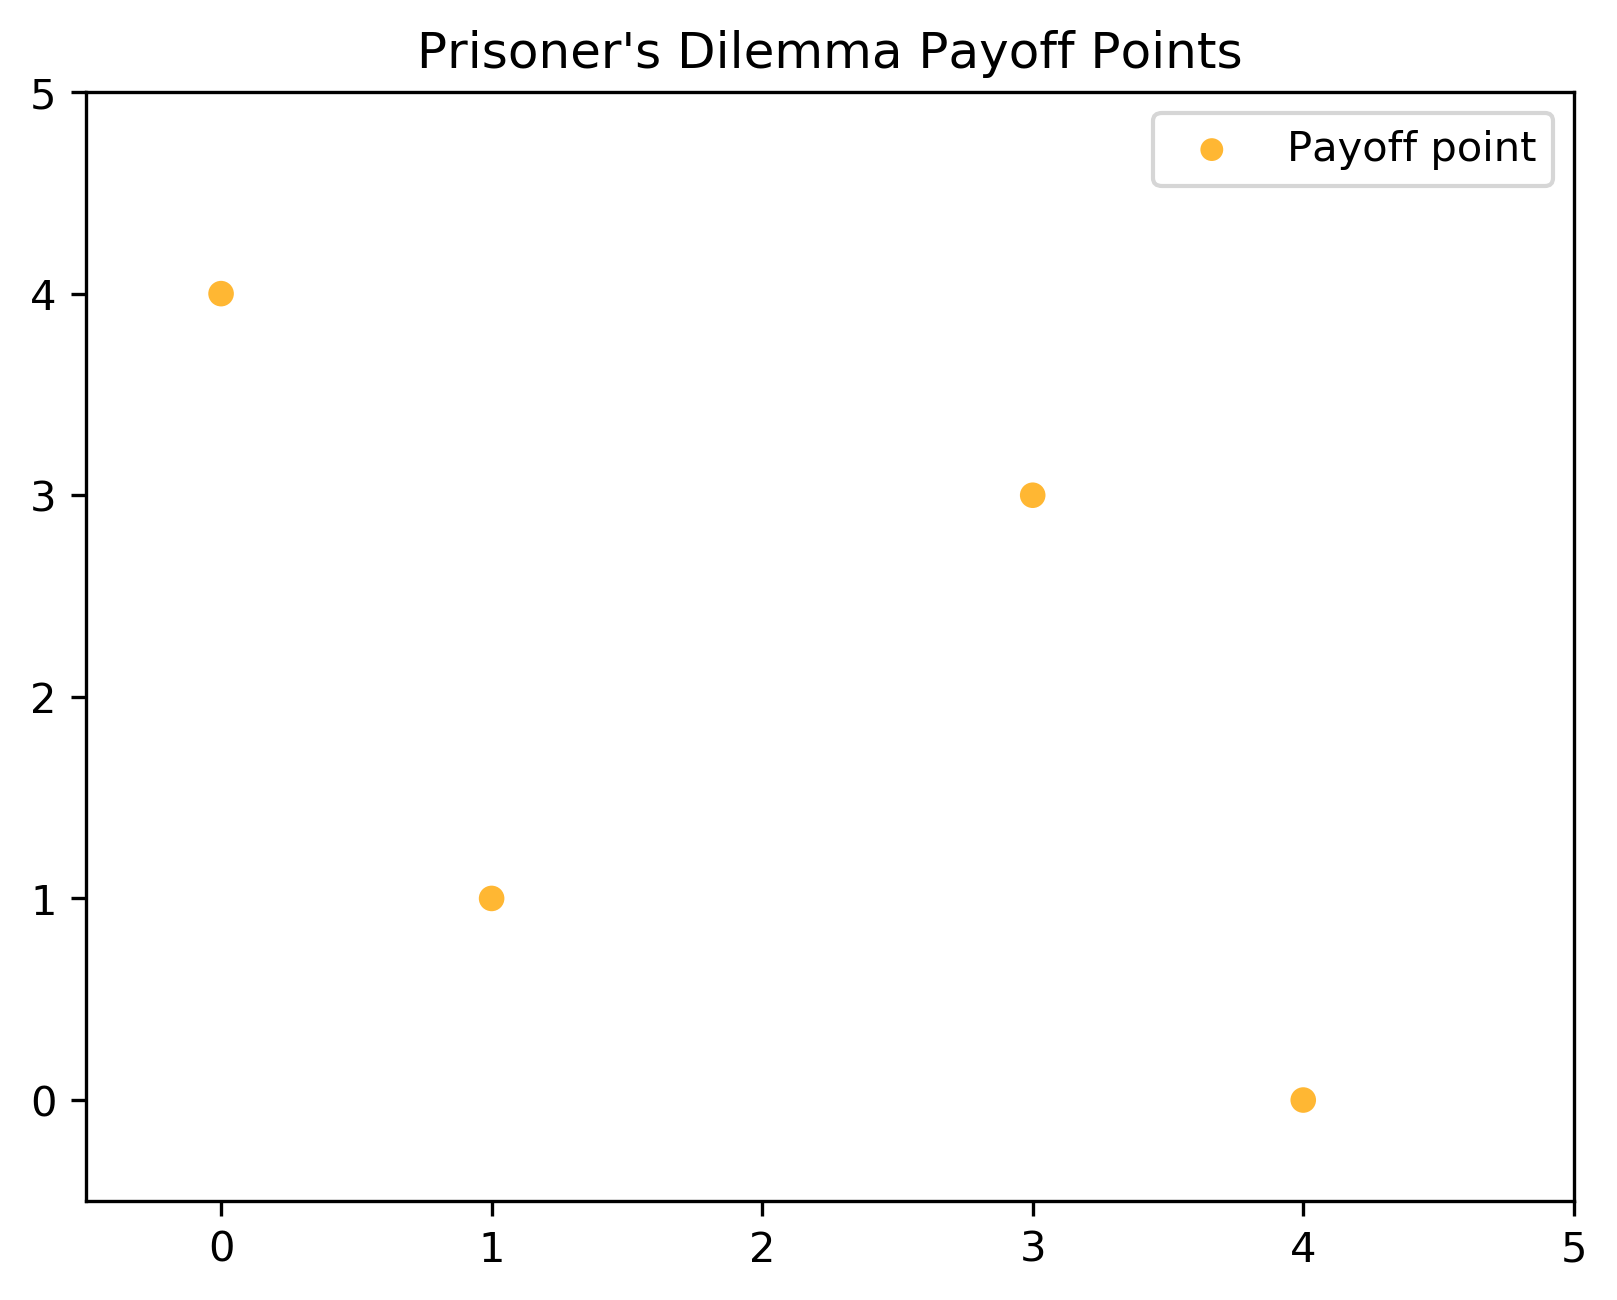
\includegraphics[scale=0.5]{resources/prisoners_dilemma_payoffs.png}
	\caption{The payoff points in a prisoner's dilemma game.}
	\label{prisoners_payoff_plot}
\end{figure}

\np The fact that limited invasions occur in this scenario makes sense when several facts about the model are considered:
\begin{enumerate}[label=(\alph*)]
	\item mutations can occur anywhere within the space and are small.
	\item the fitness of the individuals (resident and mutant) is equal in areas of the surface not affected by the mutation.
	\item for a mutant to invade, they must achieve a fitness \textit{greater} than that achieved by the resident - as opposed to greater than or equal to.	
\end{enumerate} 
\np
So, if a mutation occurs at the point (2, 2), given that this mutation has a relatively small radius, 
the expected payoff of the mutant will not differ from that of the resident because the mutation does not touch any of the payoff points.
Hence, the fitnesses are equal, and no invasion occurs.
Running simulations using this model results in `utility surfaces' that seem to have a evolved to play the prisoner's dilemma defined above,
rather than evolving towards a surface that is meaningful in general.

\todo{distance/fitness measure of prisoner's dilemma run}

\np So, while our source material tends to equivocate in regard to what kinds of games are played,
a dynamically evolving system shows that evaluating individual fitnesses using performance in only one kind of game 
does not generate meaningful results. Next, we focus on a  measure in which fitness is based upon the individual's aggregated performance across many games.

\paragraph{Many-Game Fitness Measure}
\np We move to a discussion of the results generated by simulations that measure fitness as an average of the payoff earned by individuals across many symmetric games.
Now, the games that individuals play in determining fitness contain payoffs as described in \ref{a_through_d}, where $a$ through $d$ are independent and identically distributed random variables.
Leading on from our note in the preceding that single-game fitness leads to an exorbitantly high number of mutations that do not lead to an invasion, analogously, 
localised mutations and randomly sampled games is computationally very inefficient. So, we first look at a more efficient sampling mechanism before discussing our main result.

\np Sampling many symmetric games creates a payoff-point plot that is symmetric about the line of equality and the line of equality is heavily sampled relative to the rest of the space.
This is because two of the four payoff points in each sampled game fall on the line of equality.
If we imagine the payoff-point plot (e.g. figure \ref{prisoners_payoff_plot}) as being a top-down view of one of our utility surfaces,
then we can randomly place a mutation amongst the sampled payoff-points to visualise the amount of waste that occurs when sampling like this.
Figure \ref{symmetric_payoff_plot} shows a randomly sampled mutation plotted amongst payoff-points of 40 randomly sampled games.
\begin{figure}
	\centering
	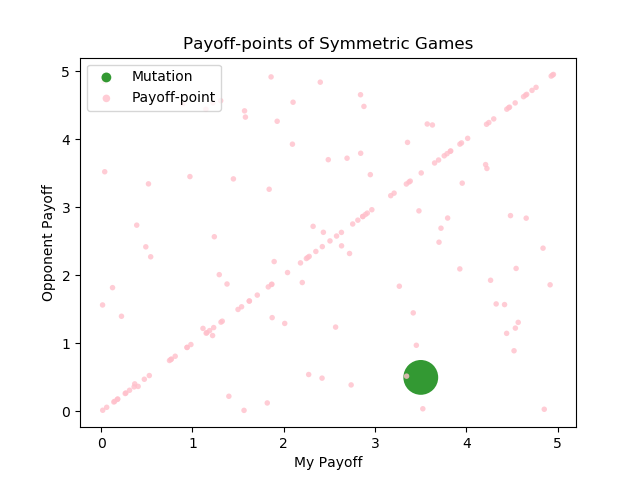
\includegraphics[scale=0.7]{resources/scatter_symmetric_mutation.png}
	\caption{Payoff-points of 40 randomly sampled games.}
	\label{symmetric_payoff_plot}
\end{figure}
We can see that of the 160 payoff points in the sample, only one occurred in the area of the mutation.
The rest of the payoff points will not contribute to a difference in fitness between the resident and mutant and so are a waste of computational resources.
We develop a more efficient sampling technique.
In this technique, two of the four payoff points in a symmetric-game still occur along the line of equality,
but the other two in each game are sampled from close to the mutation.
The payoffs $a$ through $d$ are sampled from the following, where $\mu$ is the centre of the mutation and $\delta$ is some constant linked to the radius of the mutation.
\begin{center}\label{local_a_through_d}	
	$a \sim U(0,\phi) \qquad a \in I$
	
	$b \sim \mu \pm U(0,\delta) \qquad b \in I$
	
	$c \sim \mu \pm U(0,\delta) \qquad c \in I$
	
	$d \sim U(0,\phi) \qquad d \in I$
\end{center}


\noindent Figure \ref{local_symmetric_payoff_plot} is an example of a sample of 40 games in which the payoffs are sampled using this technique.
It can be seen that payoff-points are now concentrated around the area that the mutation occurs so will contribute to a difference in fitness.
This technique means that every game will have at least one payoff-point that touches the mutation area.
This technique introduces no additional bias into the model: it is as if we freely sample payoffs from the whole space and then filter out the ones that do not have an effect on eventual fitness comparison.

\begin{figure}
	\centering
	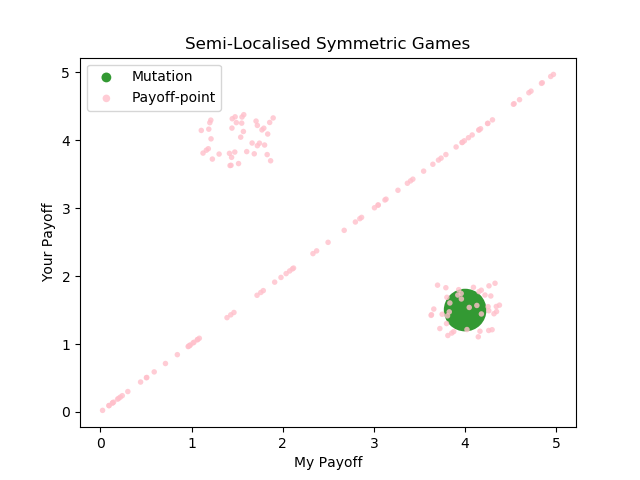
\includegraphics[scale=0.7]{resources/localised_symmetric_game_mutation.png}
	\caption{Payoff-points of 40 `locally' randomly sampled games.}
	\label{local_symmetric_payoff_plot}
\end{figure}

\chapter{Conclusion}


\todo{is this to speculative/waffley?}
Intuitively, the non-meaningful results achieve when sampling only one kind of game fit with our analogy of the utility function in some way representing the real-world preferences of some agent.\
In reality, agents face many more kinds of situations than just one instance of a prisoner's dilemma,
and so to generate a utility function that is potentially recognisable as one of a real-world agent the function will need to be resilient to many different situations.

\bibliography{thesis}
\bibliographystyle{apalike}

\end{document}